Sensitivity analysis identifies how the variation of model input
parameters affect select performance 
metrics of the fuel cycle. Additionally, it reveals the combined effect 
of varying multiple parameters on 
an output metric. This information is then used to design 
an optimized transition scenario by identifying which input parameters 
will affect the results the most, and how these parameters should be 
changed to obtain desired results (e.g., minimizing \gls{HALEU} requirements
of a transition). 

\section{Methodology}
The analysis was performed on Scenario 7 and Scenario 
14 to provide insight into how the input parameters affect the output 
metrics for both a once-through and recycle fuel cycle. 

\Cyclus was coupled to Dakota \cite{adams_dakota_2019},
and Dakota is the driver for the analysis. This coupling mirrors  
the scripts in the \texttt{dcwrapper} GitHub repository \cite{chee_arfcdcwrapper_2019}.
Three different types 
of sensitivity analysis were performed: \acrfull{OAT}, synergistic, 
and global. \gls{OAT} analysis varies a single input parameter to 
investigate the effect of each parameter individually. In the context of 
this work, synergistic 
analysis varies two input parameters at once to investigate how the 
interaction of the two parameters affects the results. Finally, the global 
analysis varies more than two input parameters to provide a holistic 
view of how multiple parameters interact and affect the output metrics. 

The input parameters varied include the transition 
start time, the build share of each type of advanced reactor, 
the \gls{LWR} lifetime, and the discharge burnup of fuel from the 
\gls{HALEU}-fueled reactors. The transition start time ranges from January 
2025 to January 2040 in three-month intervals, but the same energy demand 
will be specified for all perturbations (87.20 GWe-yr). The build share 
variable will be repeated three times (for varying the build share of each 
type of advanced reactor) with build share percentages ranging from 0-50\% 
in increments of 5\%. To account for the build share of an advanced reactor
the deployment scheme described in Section \ref{sec:once-through-methods}
was adjusted. Instead of the reactor type with the largest power output 
deployed first, the reactor with the specified build share is deployed first 
until the build share is met. Then the remaining two reactor types are 
deployed in the manner described in Section \ref{sec:once-through-methods},
with the larger of the two reactors preferentially deployed and the smaller 
reactor deployed last to meet the power demand. Figure \ref{fig:build-share-deploy}
illustrates how this deployment scheme is applied to meet a demand of 530 
MWe and a VOYGR build share of 50\%. 

\begin{figure}
    \centering 
    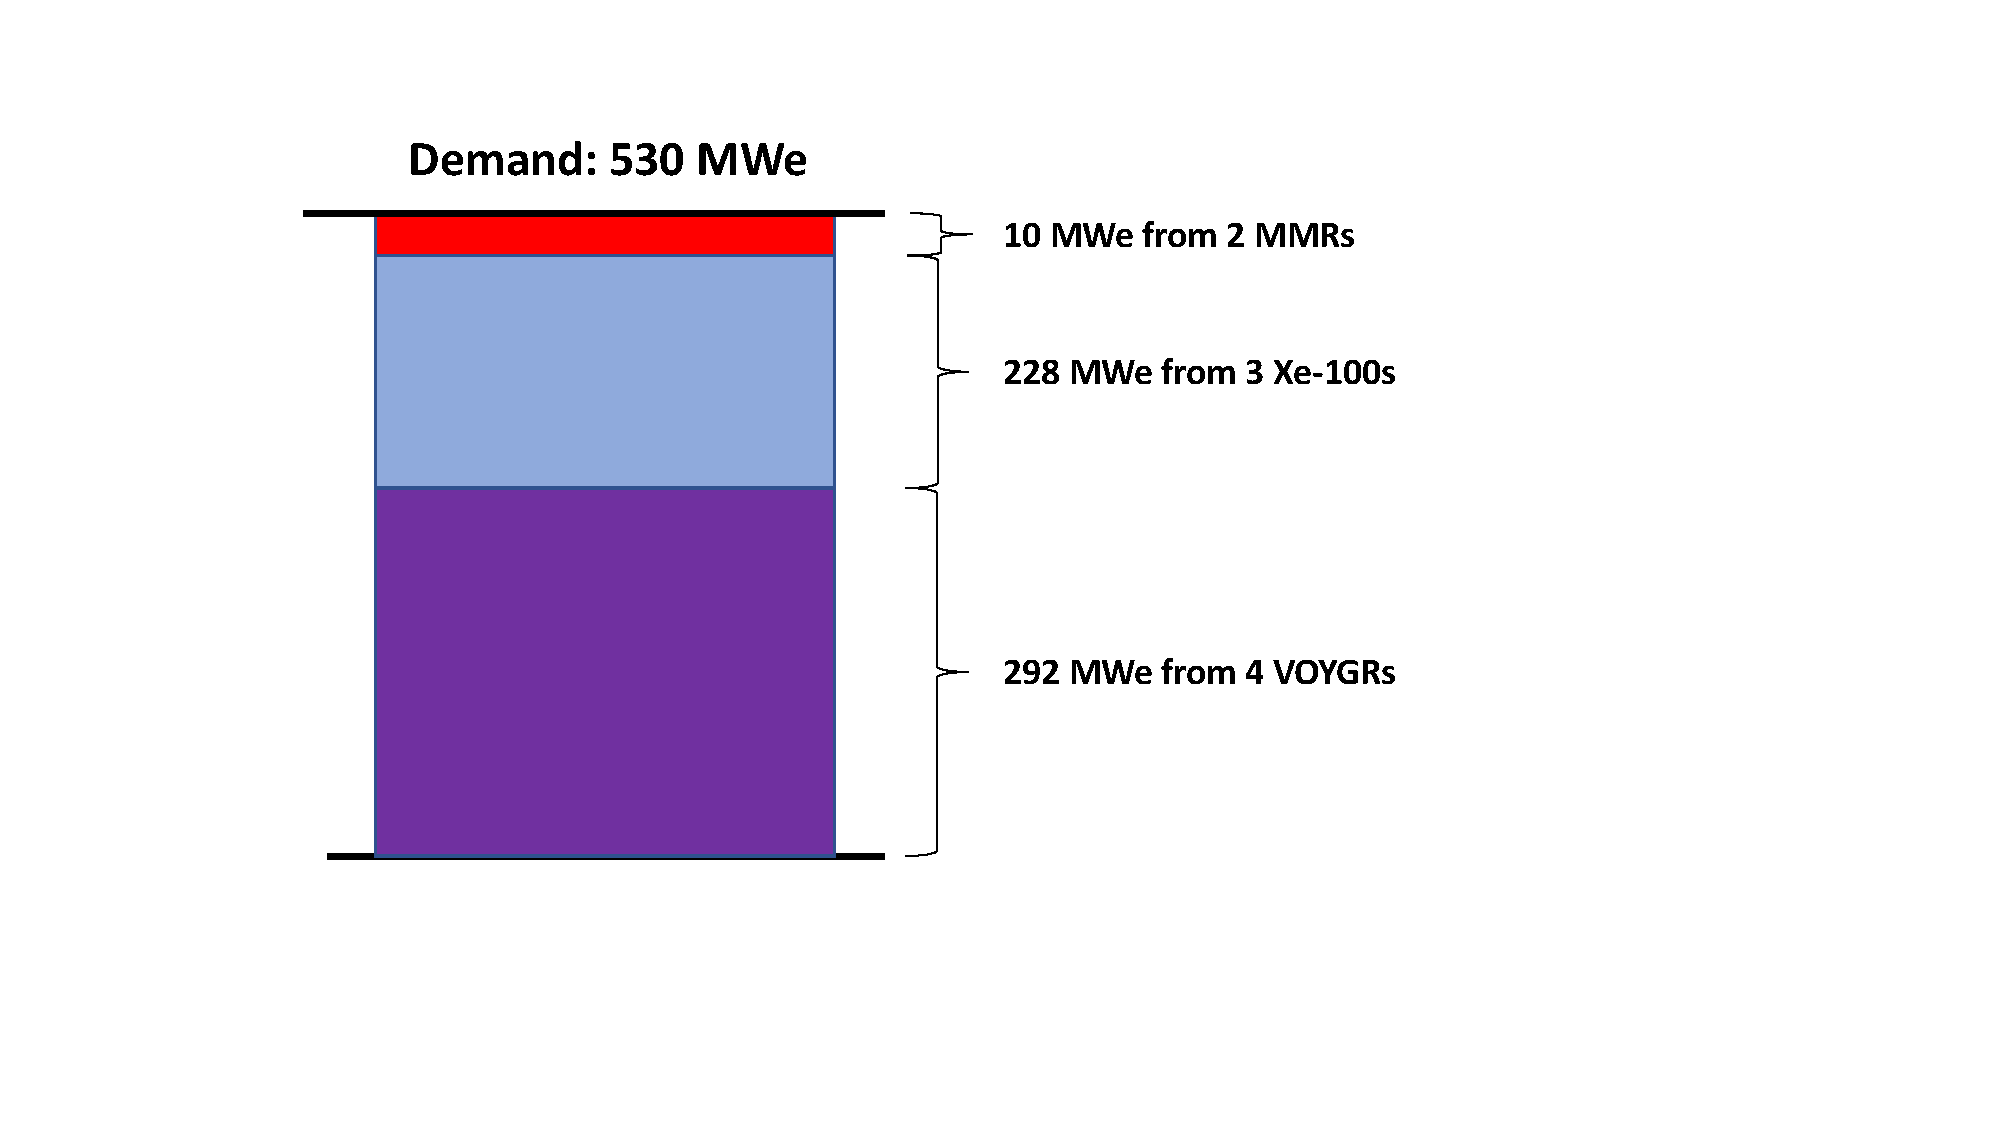
\includegraphics[scale=0.45, trim=50 100 100 0,clip]{VOYGR_build_share.pdf}
    \caption{Demonstration of the adjusted advanced reactor deployment 
    scheme to meet a demand of 530 MWe and a VOYGR build share of 
    50\%.}
    \label{fig:build-share-deploy}
\end{figure}

The \gls{LWR} lifetimes are varied based 
on the percent of the fleet that operate for 60 and 80 years. This 
variable will vary between 0-50\% of the \gls{LWR} fleet operating for 80 
years, while the other \glspl{LWR} operate for 60 years. The 
\glspl{LWR} do not all start operation at the same time, so the 
selection of the \glspl{LWR} that operate for 80 years affects the results, 
even if the number is the same. Therefore, reactors will be selected for 
operation to 80 years in 
descending order of power output, reflecting the greater likelihood of 
larger units receiving a license extension. Previous sensitivity analysis of 
fuel cycle transitions considered the impact of the transition start time 
and the \gls{LWR} lifetimes \cite{chee_sensitivity_2019,feng_sensitivity_2020},
which forms the basis for why these input parameters were selected for this 
work.

Variations of the discharge burnup of each \gls{HALEU}-fueled reactor (the 
Xe-100 and \gls{MMR}) were carried out slightly differently. Variation 
of this parameter is being done because these reactors are aiming to achieve 
burnup values that are much higher than what the NRC has approved fuel for 
\hl{Citation?}. Therefore, inclusion of this variable explores the impact 
on resource needs for if these reactors are not able to achieve their 
reported burnup values. This analysis is not performed for the VOYGR because this 
design aims to achieve a burnup that the NRC is comfortable with. 

To vary the burnup of the Xe-100, two different systems were enacted. The 
first was to vary the number of passes each pebbles goes through the core
while keeping the length of each pass and the total mass of uranium 
in the core constant. Varying the number of passes between two and six 
results in discharge burnup values of 56, 84, 112, 140, and 168 MWd/kgU, 
using Eq. \ref{eq:fuel_mass}. The second system was to vary the length 
of each pass while keeping the number of passes and the total mass of uranium 
constant. The goal of the second system is to cause a small change in the 
discharge burnup to examine how a smaller change in the burnup affects 
the resource needs. This system results in burnup values of 151 and 185 MWd/kgU, 
which are about $\pm$10\% of the stated discharge burnup of 168 MWd/kgU. 

To vary the burnup of the \gls{MMR} the cycle time, and thus lifetime, of 
the reactor was varied while the total mass of uranium was held constant. 
Cycle times of 10, 15, and 20 years were considered, resulting in burnup 
values of 41, 62, and 82 MWd/kgU. Additionally, the lifetime was varied to 
result in burnup values $\pm$10\% and $\pm$5\% around the stated burnup of 
82 MWd/kg, resulting in burnup values of 74, 78, 86, and 90 MWd/kgU. 

The output metrics of 
interest for this analysis include the amount of waste generated that 
must be sent to a repository (\gls{SNF} mass), the mass of enriched uranium, 
the mass of \gls{HALEU},
the amount of \gls{SWU} capacity required to produce all enriched uranium, the 
\gls{SWU} capacity required to produce \gls{HALEU}, and the feed uranium 
required to produce \gls{HALEU}. Each metric will be evaluated based on the 
cumulative sum required, starting at the transition start time. Previous 
sensitivity analysis of fuel cycle transitions considered the waste 
discharged, \gls{SWU} 
capacity required, and natural uranium requirements
\cite{richards_application_2021,feng_sensitivity_2020} 


\section{One-at-a-time}
\subsection{Scenario 7}
This section discusses the results of the \gls{OAT} sensitivity analysis 
as applied to Scenario 7. A subsection of this analysis is presented 
in \hl{Cite ANS Paper}, but the analysis presented here has an expanded scope. 
Additionally, the work presented here uses an updated deployment scheme to 
account for non-consistent replacement of advanced reactors identified in 
\hl{ANS Paper}. The results discuss
the relative change in each metric for each parameter varied. The minimum, 
average, and maximum value for each metric is provided in Table 
\ref{tab:oat_values}.

\begin{table}
    \centering
    \caption{Minimum, average, and maximum value of each metric caused 
    by the variation of each parameter.}
    \label{tab:oat_values}
    \begin{tabular}{llrrr}       
        \hline 
        Parameter &     Metric &      Minimum &      Average &      Maximum \\\hline
        Transition Start &  Fuel Mass & 2.832004e+07 & 3.001442e+07 & 3.085691e+07 \\
                         & HALEU Mass & 2.777396e+07 & 2.931392e+07 & 3.005491e+07 \\ 
                         &  Total SWU & 9.727160e+08 & 1.035603e+09 & 1.067644e+09 \\ 
                         & HALEU SWU & 9.690305e+08 & 1.030876e+09 & 1.062295e+09 \\
                         &        SNF & 2.600173e+07 & 2.743657e+07 & 2.812741e+07 \\  
                         & HALEU Feed & 8.406729e+08 & 8.936249e+08 & 9.204018e+08 \\\hline
        LWR Lifetimes &  Fuel Mass & 2.226230e+07 & 2.574361e+07 & 2.933547e+07 \\
                      & HALEU Mass & 2.186991e+07 & 2.527842e+07 & 2.884623e+07 \\
                      &  Total SWU & 7.779876e+08 & 8.972582e+08 & 1.021053e+09 \\
                      &  HALEU SWU & 7.753394e+08 & 8.941187e+08 & 1.017751e+09 \\
                      &        SNF & 1.955625e+07 & 2.305043e+07 & 2.668538e+07 \\
                      & HALEU Feed & 6.715754e+08 & 7.746336e+08 & 8.819633e+08 \\\hline 
        Xe-100 Build Share &  Fuel Mass & 8.228834e+07 & 1.130189e+08 & 1.471439e+08 \\
                           & HALEU Mass & 2.826681e+06 & 1.077601e+07 & 1.803929e+07 \\
                           &  Total SWU & 1.082813e+09 & 1.089912e+09 & 1.101530e+09 \\
                           &  HALEU SWU & 1.275350e+08 & 3.998760e+08 & 6.501138e+08 \\
                           &        SNF & 7.510853e+07 & 1.032204e+08 & 1.344031e+08 \\
                           & HALEU Feed & 1.081440e+08 & 3.448436e+08 & 5.622094e+08 \\\hline 
        MMR Build Share &  Fuel Mass & 3.701890e+07 & 4.917833e+07 & 6.134049e+07 \\
                        & HALEU Mass & 2.670288e+07 & 3.851759e+07 & 5.039230e+07 \\
                        &  Total SWU & 9.901021e+08 & 1.599871e+09 & 2.211838e+09 \\
                        &  HALEU SWU & 9.204794e+08 & 1.527922e+09 & 2.137948e+09 \\
                        &        SNF & 3.439781e+07 & 4.065525e+07 & 4.688864e+07 \\
                        & HALEU Feed & 7.995188e+08 & 1.309634e+09 & 1.821949e+09 \\\hline 
        VOYGR Build Share &  Fuel Mass & 3.044985e+07 & 6.435525e+07 & 9.510189e+07 \\
                          & HALEU Mass & 1.515573e+07 & 2.233175e+07 & 3.044985e+07 \\
                          &  Total SWU & 1.076518e+09 & 1.082445e+09 & 1.092329e+09 \\
                          &  HALEU SWU & 5.527729e+08 & 7.988284e+08 & 1.079883e+09 \\
                          &        SNF & 2.764653e+07 & 5.870293e+07 & 8.679207e+07 \\
                          & HALEU Feed & 4.774801e+08 & 6.913159e+08 & 9.353306e+08 \\\hline 
        Xe-100 Burnup &  Fuel Mass & 2.760515e+07 & 5.887765e+07 & 1.591116e+08 \\
                      & HALEU Mass & 2.681265e+07 & 5.808515e+07 & 1.583191e+08 \\
                      &  Total SWU & 9.558796e+08 & 2.033879e+09 & 5.489061e+09 \\
                      &  HALEU SWU & 9.505310e+08 & 2.028530e+09 & 5.483713e+09 \\
                      &        SNF & 2.486320e+07 & 5.613569e+07 & 1.563697e+08 \\
                      & HALEU Feed & 8.233245e+08 & 1.759663e+09 & 4.760799e+09 \\\hline 
        MMR Burnup &  Fuel Mass & 3.064950e+07 & 3.123978e+07 & 3.292776e+07 \\
                   & HALEU Mass & 2.985700e+07 & 3.044728e+07 & 3.213526e+07 \\
                   &  Total SWU & 1.058714e+09 & 1.085347e+09 & 1.161506e+09 \\
                   &  HALEU SWU & 1.053366e+09 & 1.079998e+09 & 1.156157e+09 \\
                   &        SNF & 2.790754e+07 & 2.849783e+07 & 3.018581e+07 \\
                   & HALEU Feed & 9.128300e+08 & 9.354133e+08 & 9.999926e+08 \\
        \hline
    \end{tabular}
\end{table}


\subsubsection{Transition start time}
Delays in the transition start time generally decrease all of the output 
metrics, as shown in Figure \ref{fig:ts_scenario7}. This results matches 
expectations, because if the advanced reactors are deployed for less time, 
then they require fewer resources. However, there are some increases in 
the output metrics between individual time steps. For example, a transition 
start time of October 2029 increases the fuel mass and \gls{SNF} mass 
relative to July 2029. This increase is the result of changes in the number 
of each advanced reactor deployed, because of differences in the gap 
between energy produced and energy demand that must initially be filled when 
advanced reactors are deployed. By waiting until October 2029, more VOYGRs 
are deployed than when the transition starts in July 2029. As discussed in 
Chapter \ref{ch:once_through_results}, the VOYGR needs a larger fuel mass, 
and thus discharges more \gls{SNF} than the Xe-100 and \gls{MMR}. Therefore, 
these two metrics increase for this particular transition start time. 

\begin{figure}
    \centering
    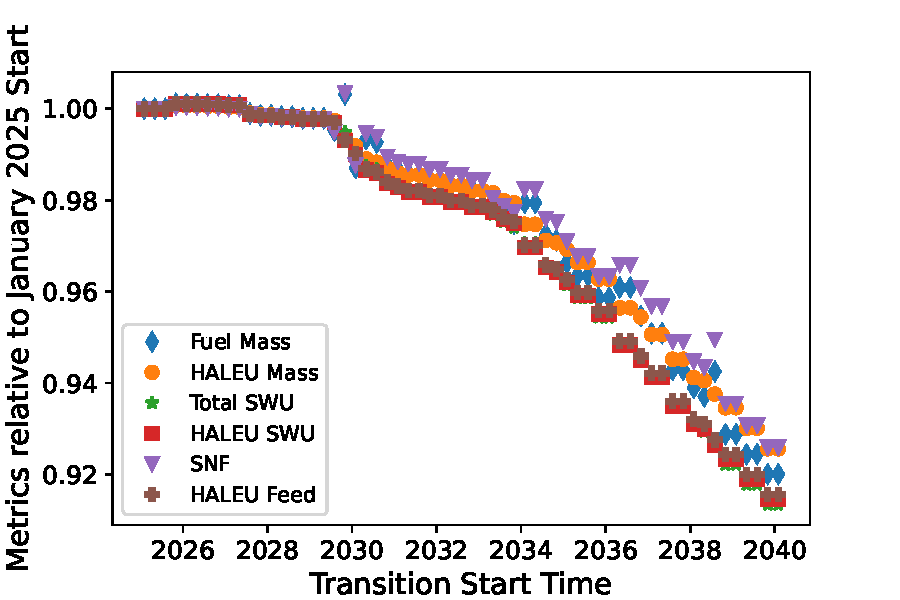
\includegraphics[scale=0.8]{ts.pdf}
    \caption{Change in each metric as a function of transition start 
    time, relative to a transition start in January 2025.}
    \label{fig:ts_scenario7}
\end{figure}

The \gls{HALEU} mass required for these transitions varied between 27.8-30.9
MTU. 

One of the disadvantages in delaying the transition start time is the 
increasing gap between energy supplied and energy demand as the transition 
start time is delayed. All of these scenarios have a constant demand 
of 87.20 GWe-yr beginning in 2025. By delaying the transition start time 
to after September 2025 (the observed initial deployment time of advanced 
reactors in Section \ref{sec:nogrowth_reactors}) there is some gap between 
the energy supplied and the energy demand. The largest gap observed is 36.7
GWe-yr, when reactors are deployed starting in January 2040. This difference 
between energy supplied and energy demand is a disadvantage of delaying 
the start time to reduce material requirements. 

\subsubsection{LWR lifetimes}
The next metric varied is the percent of the \glspl{LWR} that operate for 
80 years, reflecting a license extension. As the percent of the \gls{LWR} 
fleet operating for 80 years increases all of the metrics decrease, as 
Figure \ref{fig:lwr_scenario7} shows. All of the metrics decrease by a similar 
magnitude, with some variation because of changes in the number of each advanced 
reactor deployed, as previously discussed. The \gls{SNF} mass decreases more 
than the other metrics across this parameter space, ranging between 
19.5-26.7 MTU.

\begin{figure}
    \centering
    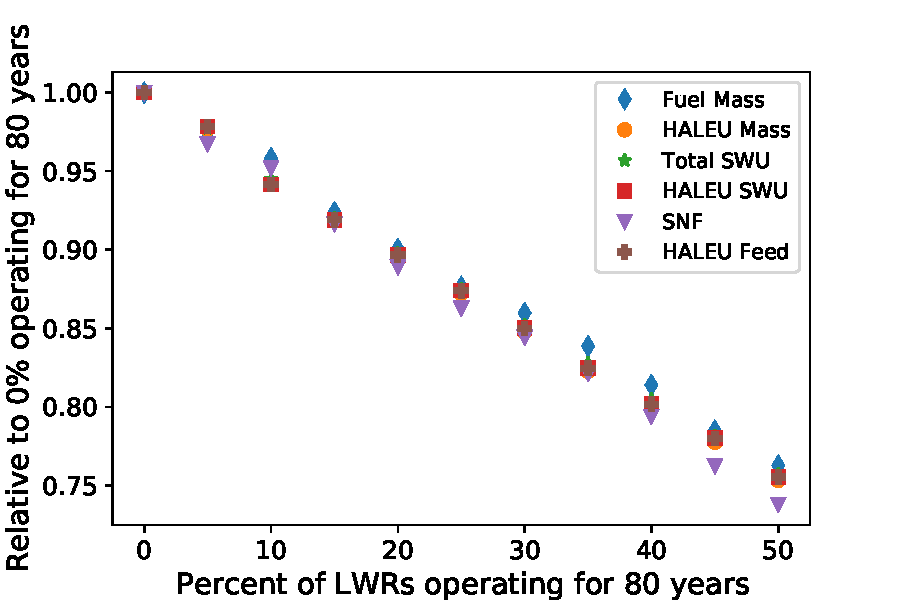
\includegraphics[scale=0.8]{lwr.pdf}
    \caption{Change in each metric as a function of percent of LWR fleet  
    operating for 80 years, relative to 0\%.}
    \label{fig:lwr_scenario7}
\end{figure}

Across this parameter space, the metrics decrease by a greater fraction than 
when varying the transition start time. The increased impact on the metrics 
is partly because the \glspl{LWR} that don't operate for 80 years all operate for 
60 years when varying this parameter, but not all of the \glspl{LWR} operate for 
60 years in the initial transition analysis or when varying the transition
start time. This modeling difference, made to simplify defining the advanced 
reactor deployment schedule, does not have a large impact on the results as 
evidenced by the maximum \gls{HALEU} mass when varying the \gls{LWR} lifetimes 
being only 4.9\% lower than the maximum \gls{HALEU} mass when varying the 
transition start time. This minimal impact from the modeling difference is 
because most of the \glspl{LWR} operate for 60 years when varying the transition start 
time. Therefore, we can attribute most of the change in the metrics to the 
change in the \gls{LWR} lifetimes. In addition to causing greater change in 
the metrics, the energy demand is always met when varying the \gls{LWR} lifetimes,
which suggests that extending the lifetimes of the \glspl{LWR} is a better 
parameter to vary if one wishes to decrease material requirements of this 
transition. 

\subsubsection{Xe-100 build share}
As the Xe-100 build share increases, the \gls{HALEU}-related metrics 
increase while the total \gls{SNF} and total fuel mass decrease and the 
total \gls{SWU} capacity stays relatively constant (Figure \ref{fig:xe100_scenario7}).
As Figure \ref{fig:xe100_s7_combined_reactors} shows, as the Xe-100 build share 
increases, the number of \glspl{MMR} is relatively constant and the number of 
VOYGRs decreases. These results show that as the Xe-100 build share increases, they 
are primarily replacing power that is supplied by the VOYGRs, instead of a portion 
of each of the other advanced reactors. This replacement of VOYGRs is because 
of the deployment scheme of this work, as the VOYGR has the largest power output 
between the VOYGR and \gls{MMR}. Therefore, the VOYGR is primarily deployed when 
the Xe-100 build share is 0\%. 

\begin{figure}
    \centering
    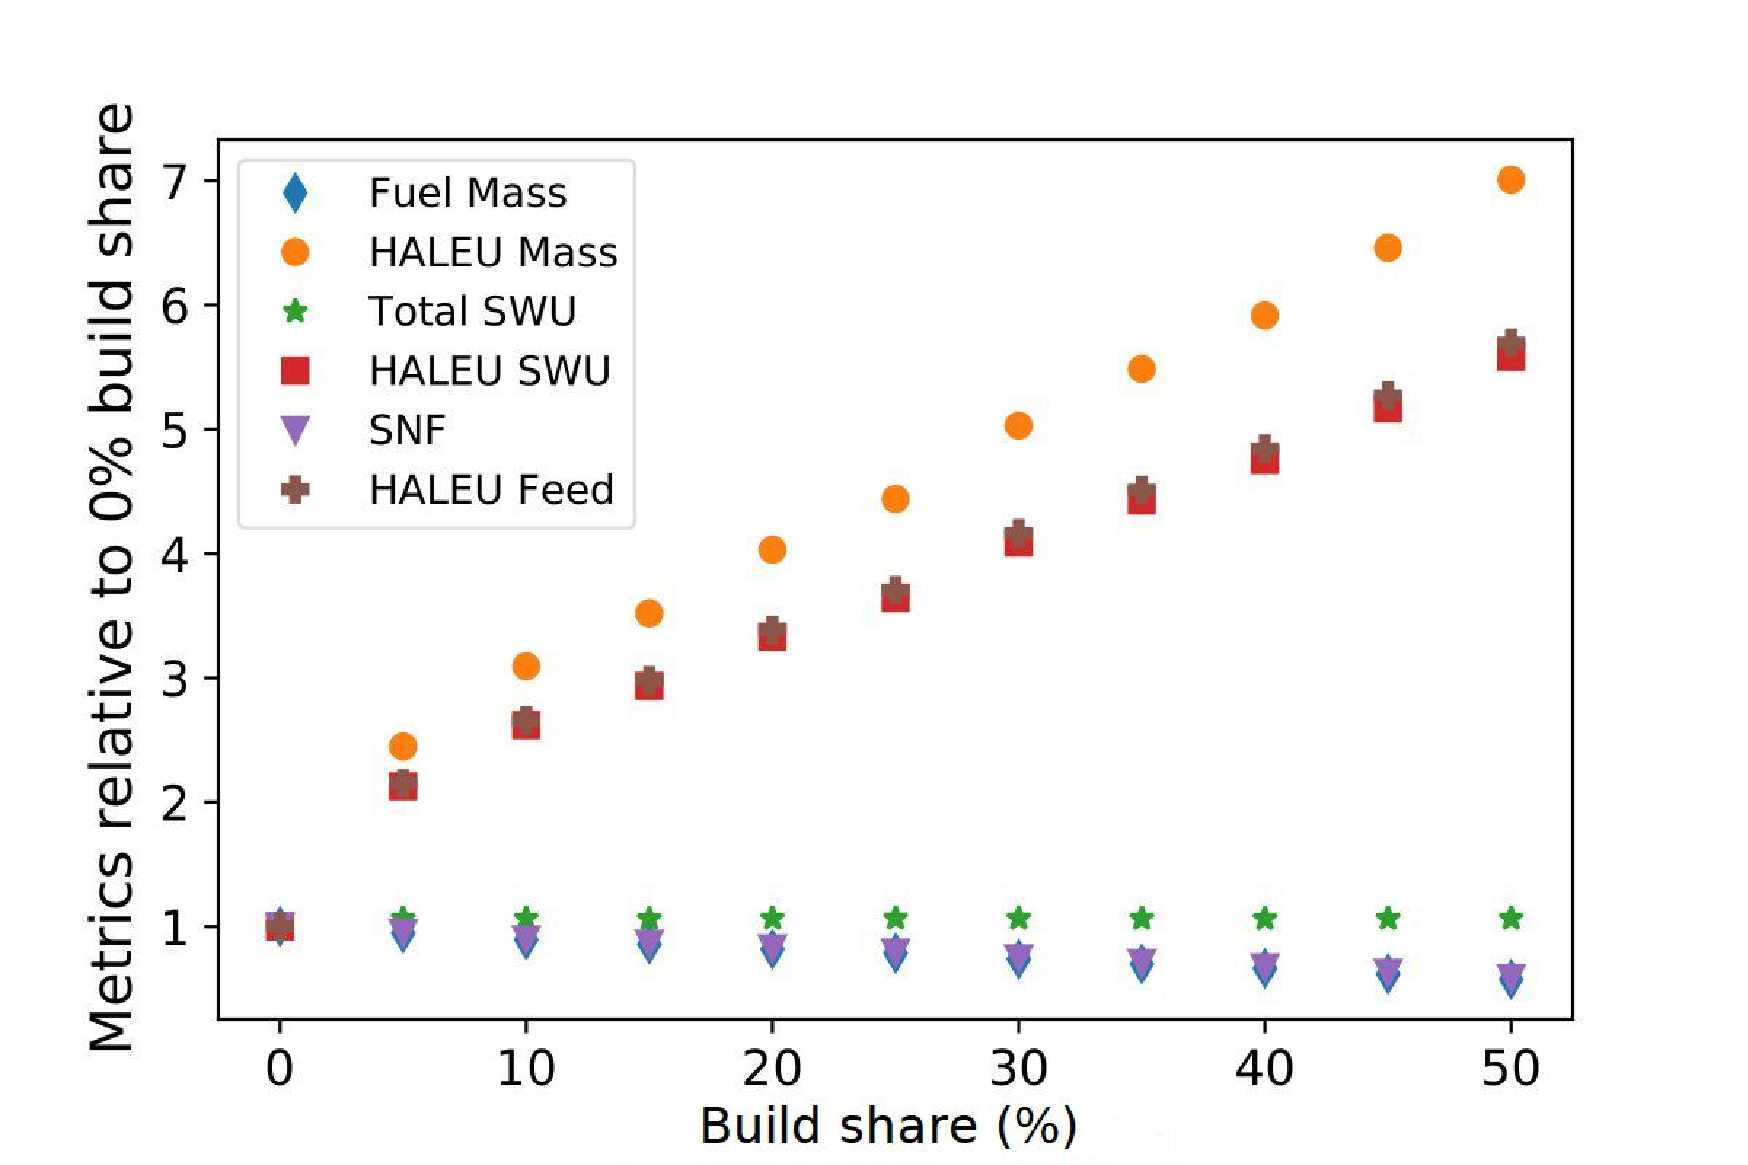
\includegraphics[scale=0.8]{xe100.pdf}
    \caption{Change in each metric as a function of Xe-100 build share, 
    relative to a build share of 0\%.}
    \label{fig:xe100_scenario7}
\end{figure}

\begin{figure}
    \centering
    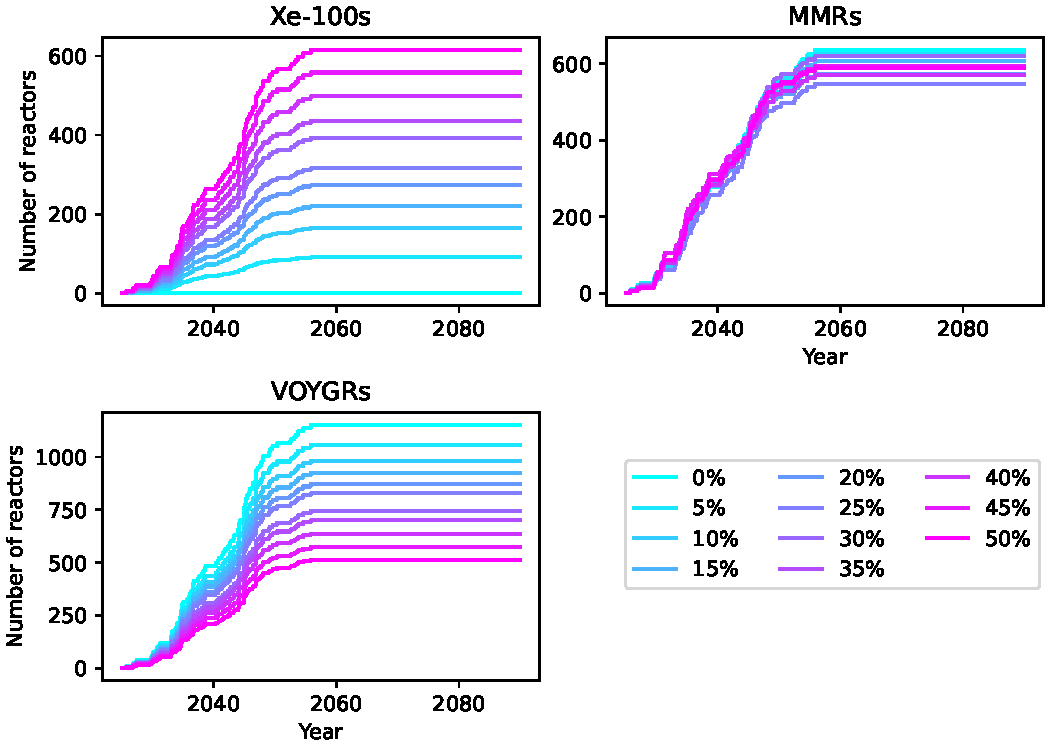
\includegraphics[scale=0.7]{xe100_combined_reactors.pdf}
    \caption{Number of Xe-100s (top left), MMRs (top right), and VOYGRs
    (bottom left) as a function of Xe-100 build share.}
    \label{fig:xe100_s7_combined_reactors}
\end{figure}

The \gls{HALEU}-related metrics increase with Xe-100 build share because more the 
power comes from advanced reactors requiring \gls{HALEU}. The total fuel mass and 
\gls{SNF} mass decrease because the Xe-100s are primarily replacing VOYGRs, and the 
Xe-100 requires less fuel per unit time and energy than the VOYGR, as discussed 
in Chapter \ref{ch:once_through_results}. The total \gls{SWU} capacity required 
is relatively constant, decreasing between 0.3-1.7\% compared to the \gls{SWU} capacity 
required for a 0\% Xe-100 build share. This stagnant behavior of the total 
\gls{SWU} capacity is consistent with the similar \gls{SWU} capacity required 
by Scenarios 3-7 in Section \ref{sec:nogrowth_swu}, when either the Xe-100 or 
VOYGR are primarily deployed. These results highlight the trade-off between the
\gls{HALEU}-related metrics and the total fuel mass and \gls{SNF} mass in deploying 
the Xe-100 versus the VOYGR. Both reactors require similar \gls{SWU} capacities, 
but because of the different product assays required the cascade configuration 
will vary. 

The \gls{HALEU}-related metrics increase to up to 538.2\% of the mass required 
for a 0\% Xe-100 build share. The total fuel mass and \gls{SNF} mass decrease 
to up to 44.11\% of the mass required for 1 0\% Xe-100 build share. 


\subsubsection{MMR build share}
As the \gls{MMR} build share increases all of the metrics increase, as shown 
in Figure \ref{fig:mmr_scenario7}. The total \gls{SWU}, \gls{HALEU} \gls{SWU}, 
and \gls{HALEU} feed have the greatest relative increase because more of the 
advanced reactor fleet uses the highest enrichment level of the three 
advanced reactors as the \gls{MMR} build share increases. The \gls{HALEU} mass 
increases with the \gls{MMR} build share because of the replacement of Xe-100s 
with \glspl{MMR} with increasing build share (see Figure \ref{fig:mmr_reactors_s7}).
The \gls{MMR} requires a greater fuel mass than the Xe-100, causing the increase 
in the \gls{HALEU} mass. The larger fuel mass required by the \gls{MMR}, compared 
with the Xe-100, compounds with the higher enrichment required by the \gls{MMR} 
to cause the greater relative increase in the total \gls{SWU}, \gls{HALEU} \gls{SWU}, 
and \gls{HALEU} feed. 

The \gls{SNF} mass does not experience the same 
relative increase as the total fuel mass because any fuel that is still in a 
reactor core at the end of the simulation is not accounted for in the 
\gls{SNF} mass. 
Based on the replacement of Xe-100s with \glspl{MMR} as the \gls{MMR} 
build share increases, these results highlight the effects of deploying the
\gls{MMR} over the Xe-100. 

\begin{figure}
    \centering
    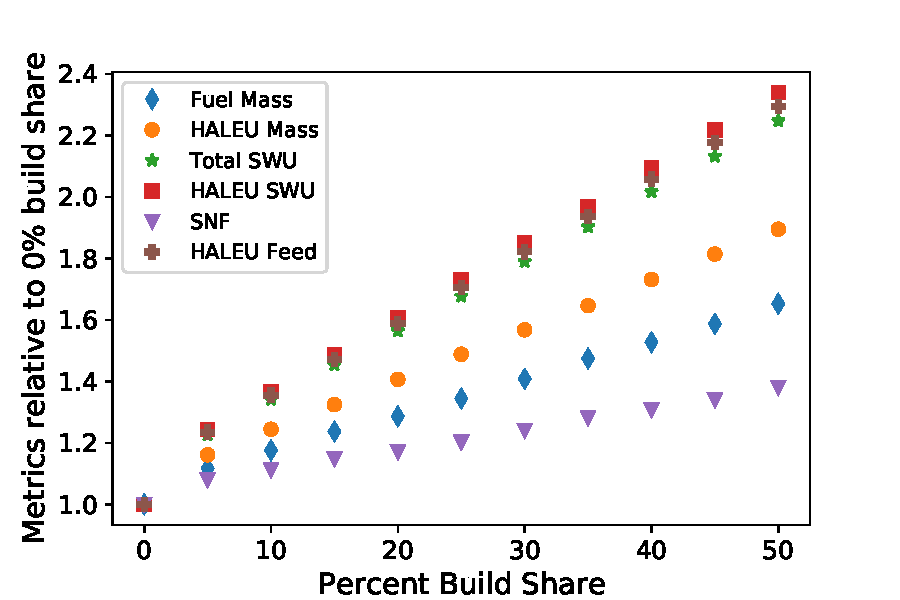
\includegraphics[scale=0.8]{mmr.pdf}
    \caption{Change in each metric as a function of MMR build share, 
    relative to a build share of 0\%.}
    \label{fig:mmr_scenario7}
\end{figure}


\begin{figure}
    \centering
    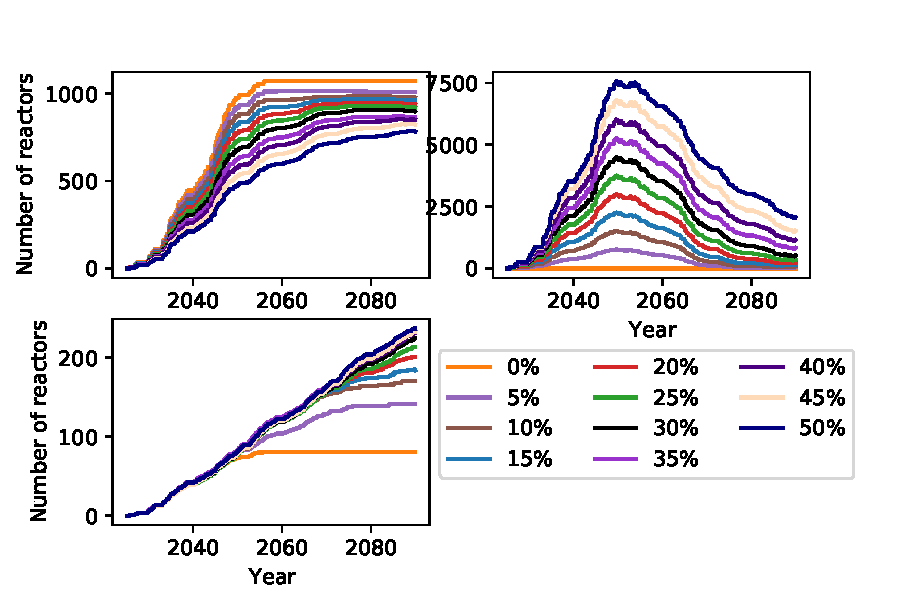
\includegraphics[scale=0.7]{mmr_combined_reactors.pdf}
    \caption{Number of Xe-100s (top left), MMRs (top right), and 
    VOYGRs (bottom left) deployed as a function of time and 
    MMR build share.}
    \label{fig:mmr_reactors_s7}
\end{figure}


\subsubsection{VOYGR build share}
When varying VOYGR build share, the impact on the metrics was 
opposite that of when varying the Xe-100 build share (Figure 
\ref{fig:voygr_scenario7}). The total fuel mass and \gls{SNF} mass 
increase, the \gls{HALEU}-related metrics decrease, and the total 
\gls{SWU} capacity remains relatively constant. This reversal 
of trends occurs because there is a replacement of Xe-100s with VOYGRs
with increasing build share (Figure \ref{fig:voygr_reactors_s7}), 
the opposite of what happens with an increasing Xe-100 build share. 

\begin{figure}
    \centering
    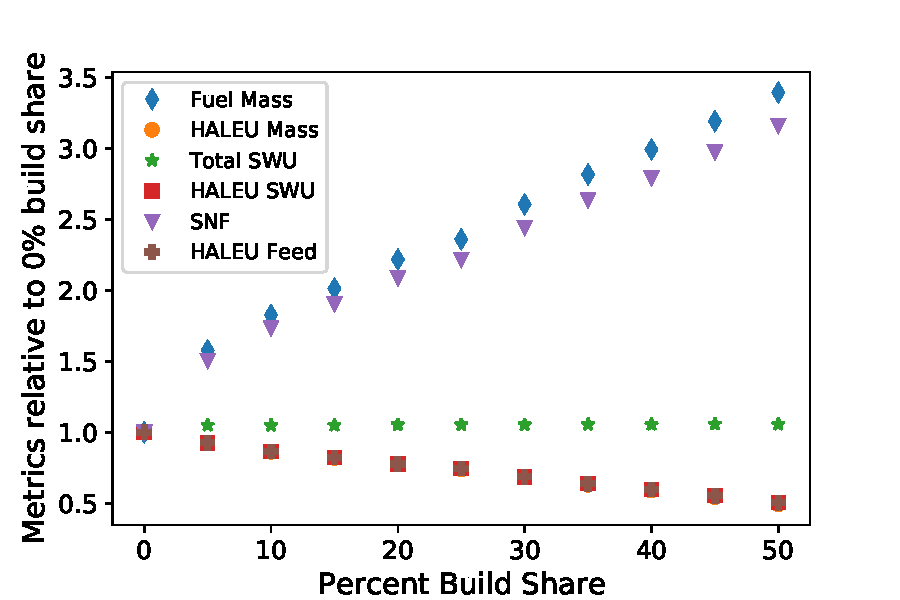
\includegraphics[scale=0.8]{voygr.pdf}
    \caption{Change in each metric as a function of VOYGR build share, 
    relative to a build share of 0\%.}
    \label{fig:voygr_scenario7}
\end{figure}

\begin{figure}
    \centering
    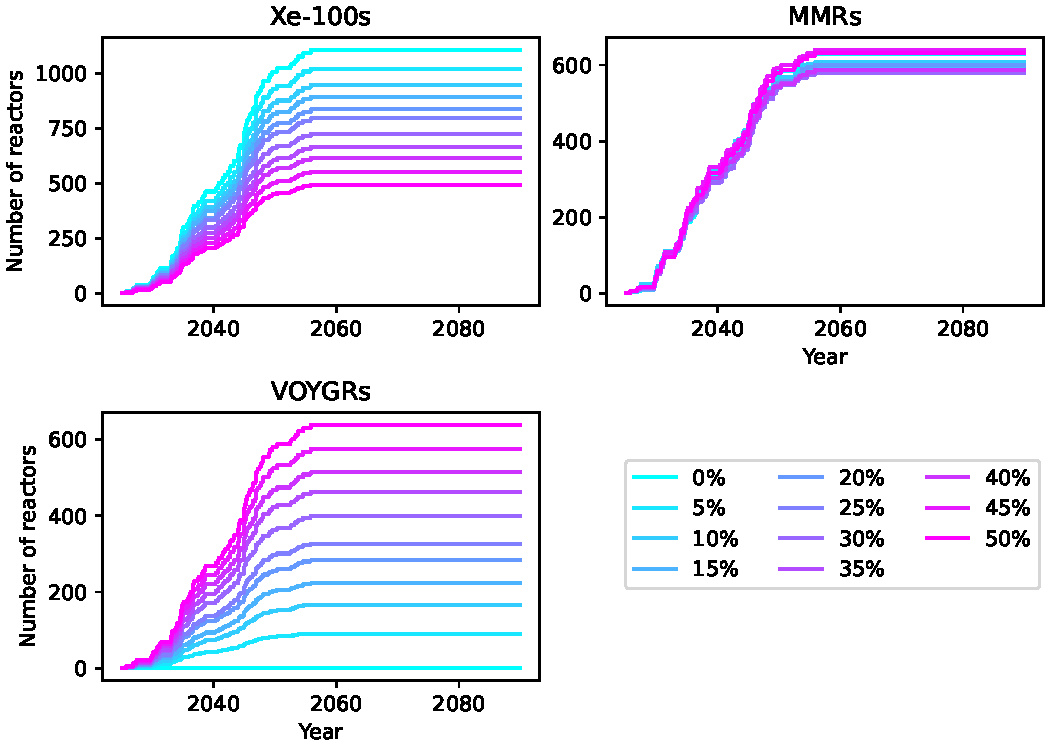
\includegraphics[scale=0.7]{voygr_combined_reactors.pdf}
    \caption{Number of Xe-100s (top left), MMRs (top right), and 
    VOYGRs (bottom left) deployed as a function of time and 
    VOYGR build share.}
    \label{fig:voygr_reactors_s7}
\end{figure}

The total \gls{SWU} capacity required varies between 99.6\%-101.2\% of the 
\gls{SWU} capacity needed for a 0\% VOYGR build share, a range of 1.077$\times 10^9$
- 1.092$\times 10^9$ kg-SWU (Table \ref{tab:oat_values}). The total fuel mass 
and \gls{SNF} mass increase 
up to 313.9\% of the mass required for a 0\% VOYGR build share, and the 
\gls{HALEU}-related metrics decrease to 49.77\% of the mass required 
for a 0\% VOYGR build share. The \gls{SNF} and total fuel masses increase 
because the VOYGR requires more fuel than the Xe-100, largely stemming from 
the difference in discharge burnup of these two reactors. The \gls{HALEU}-related 
metrics all decrease because the VOYGR does not require \gls{HALEU}, so as the 
VOYGR build share increases a smaller portion of the advanced reactor fleet 
requires \gls{HALEU}. While the trends from varying the VOYGR build share 
mirrors the trends from varying the Xe-100 build share, the magnitude of the 
changes are not the same. The magnitude difference occurs because these 
parameter variations cover adjacent but not overlapping design spaces. 

\subsubsection{Xe-100 burnup}
When varying the burnup of fuel discharged from Xe-100s, the metrics decrease 
as the burnup increases (Figure \ref{fig:xe100_bu_s7}). This decrease in material requirements because as 
the burnup is increased the fuel is going through the core more times or the 
length of each pass is longer. Therefore, the Xe-100s in the simulation are receiving 
less fuel at each refueling or receiving fuel less often as the burnup increases. 
Varying the burnup of the Xe-100 has a large impact on the metrics, up to fives times 
the material requirements compared with a burnup of 168 MWd/kgU, because most of 
the energy produced in these scenarios comes from Xe-100s and many more Xe-100s are 
deployed than \glspl{MMR} or VOYGRs. Therefore, changes to the Xe-100 refueling is 
magnified because of the greater number of the reactor deployed. 

\begin{figure}
    \centering
    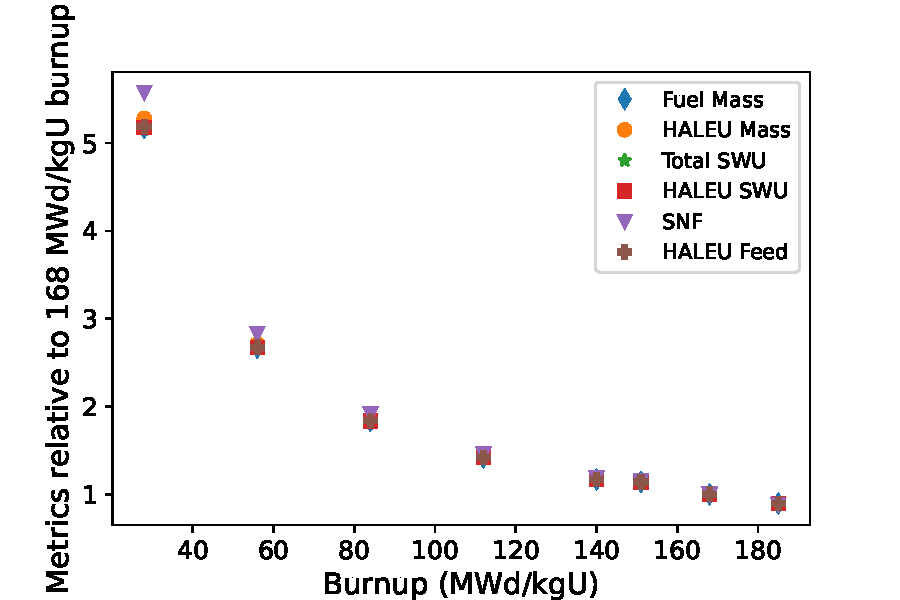
\includegraphics[scale=0.8]{xe100_bu.pdf}
    \caption{Change in metrics from varying the burnup of fuel 
    discharged from Xe-100, relative to a burnup of 168 MWd/kgU.}
    \label{fig:xe100_bu_s7}
\end{figure}

\subsubsection{MMR burnup}
When the \gls{MMR} discharge burnup is varied the metrics all decrease, similar 
to what was observed by varying the Xe-100 discharge burnup. One difference in 
the trends observed between varying these two parameters is the magnitude of 
the relative changes. Varying the \gls{MMR} burnup has a smaller relative effect 
on the metrics than varying the Xe-100 burnup because there are fewer \glspl{MMR} 
deployed in the transition. Therefore the impact on the cumulative metrics 
(what is reported here) is smaller. Another difference is that the total 
\gls{SWU}, \gls{HALEU} \gls{SWU}, and \gls{HALEU} feed increase the most 
when the \gls{MMR} burnup is low, compared with the \gls{SNF} having the 
greatest relative increase with the Xe-100 burnup is low. 

\begin{figure}
    \centering
    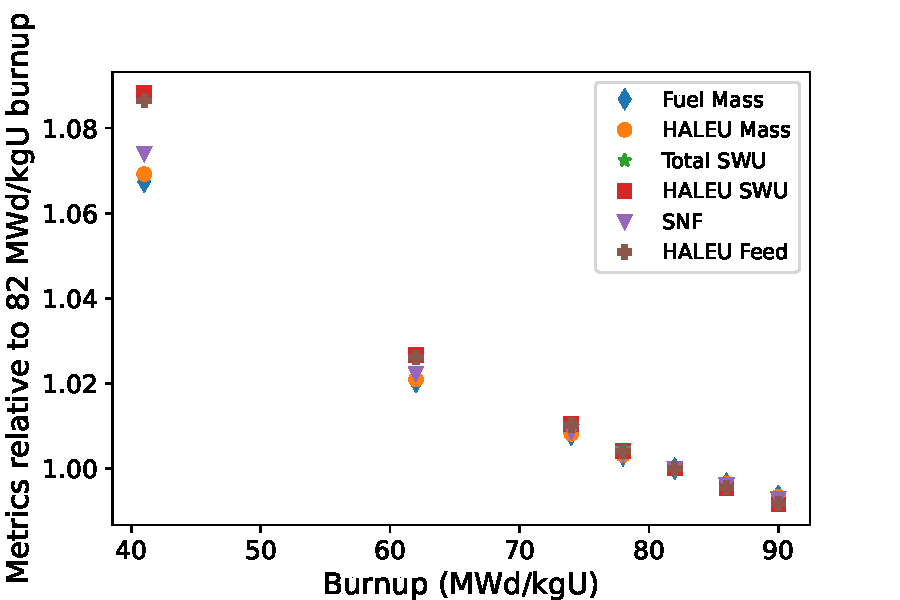
\includegraphics[scale=0.8]{mmr_bu.pdf}
    \caption{Change in metrics from varying the burnup of fuel 
    discharged from the MMR, relative to a burnup of 82 MWd/kgU.}
    \label{fig:mmr_bu_s7}
\end{figure}

\subsubsection{Burnup variations with a common build share}
To better investigate the effect of varying the discharge burnup of the Xe-100 
and \gls{MMR} without the influence of the deployment scheme preferentially
deploying Xe-100s, we repeated each set of analysis using a constant 20\% 
build share for both the Xe-100 and \gls{MMR} (VOYGRs met the remaining 60\%). 
Using a constant build share for 
both reactors means that they each will supply the same fraction of the energy demand.
However, because of the different power output for each reactor a constant build 
share does not mean that the same number of each reactor is built. 

Figure \ref{fig:bu_constant} shows the relative change in each metric as a result 
of varying the \gls{MMR} (Figure \ref{fig:mmr_bu_constant}) and Xe-100 
(Figure \ref{fig:xe100_bu_constant}) discharge burnup with the constant build 
share. Changing the \gls{MMR} burnup has a greater impact with the specified 20\% 
build share then when the build share was not specified. This change is because 
more \glspl{MMR} are deployed with a 20\% build share than when the build share is 
not specified. Conversely, the Xe-100 burnup has a smaller impact on the metrics 
with a 20\% build share than when a build share isn't specified because fewer 
Xe-100s are deployed. 

\begin{figure}
    \centering
    \begin{subfigure}{0.48\textwidth}
        \centering
        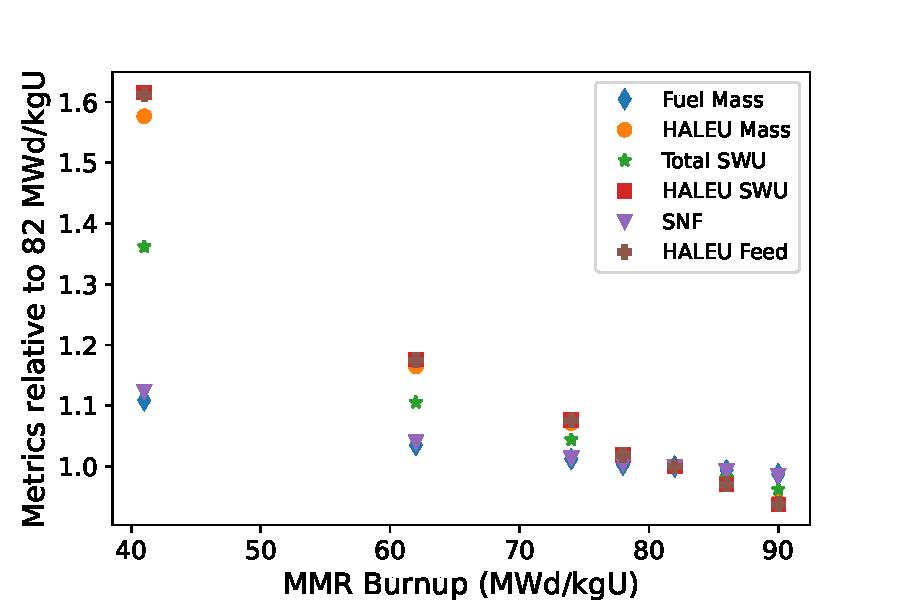
\includegraphics[width=\textwidth]{mmr_bu_constant.pdf}
        \caption{Change in metrics when varying the MMR discharge burnup, 
        assuming a constant 20\% build share for the MMR and Xe-100.}
        \label{fig:mmr_bu_constant}
    \end{subfigure}
    \hfill
    \begin{subfigure}{0.48\textwidth}
        \centering
        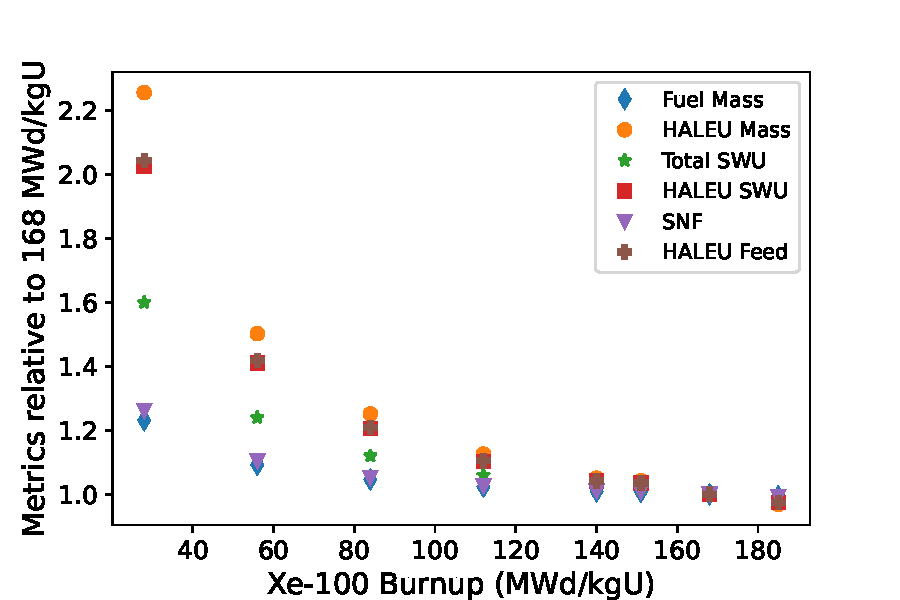
\includegraphics[width=\textwidth]{xe100_bu_constant.pdf}
        \caption{Change in metrics when varying the Xe-100 discharge burnup, 
        assuming a constant 20\% build share for the MMR and Xe-100.}
        \label{fig:xe100_bu_constant}
    \end{subfigure}
    \caption{Relative changes in the metrics caused by changes in the discharge 
    burnup of the HALEU-fueled advanced reactors, assuming a constant 
    20\% build share for the Xe-100 and MMR.}
    \label{fig:bu_constant}
\end{figure}

By applying a constant build share, variations in these parameters lead to 
more variation in the effect on the metrics than when a build share was not 
specified. In these scenarios, varying the discharge burnup of either reactor 
leads to the greatest impact on the \gls{HALEU}-related metrics while the  
total fuel mass and \gls{SNF} mass are affected the least. 
The \gls{HALEU}-related metrics are affected the most because most of the reactors 
in these scenarios are VOYGRs, which do not require \gls{HALEU}. Therefore, 
small increases in the each of the \gls{HALEU}-related metrics led to larger 
relative changes. Conversely, the total fuel mass and \gls{SNF} masses are 
affected less by changes in these parameters because the fuel and \gls{SNF} 
for the VOYGRs are constant and increase these values such that the changes 
observed cause a smaller relative change. 

\subsection{Scenario 14}

\section{Synergistic}
The synergistic analysis in this work varied two parameters at a time to 
investigate some of the combined effects of the input parameters. Synergistic 
sensitivity analysis helps to identify if the combined effect of two parameters 
has a greater impact on the metrics that when varying a single parameter. 

\subsection{Scenario 7}\label{sec:s7_synergistic}
We ran synergistic 
analysis on all combinations of two input parameters studied in the \gls{OAT} 
analysis, except combinations of two specified build shares. The
results presented here are only a small subsection of the analysis performed, 
with the remaining results in Appendix \ref{app:s7_synergistic}.

\subsubsection{LWR lifetime and VOYGR build share}
When the percent of \glspl{LWR} operating for 80 years and the VOYGR build share 
were varied, the results are consistent with the results from varying 
each of the parameters by themselves. The effect on the \gls{HALEU} mass 
(Figure \ref{fig:lwr_voygr_share_enr_u}) is fairly uniform across the 
parameter space. As the VOYGR build share and percent of \gls{LWR} with 
extended licenses increase the \gls{HALEU} mass required decreases, 
which is consistent with the results of the \gls{OAT} analysis for these 
parameters. By combining these two parameters, there is a greater 
decrease in the \gls{HALEU} mass than the decrease observed by just varying 
a single parameter. The other \gls{HALEU} metrics, the \gls{HALEU} \gls{SWU} 
and \gls{HALEU} feed, als decrease in a similar manner as the \gls{HALEU} mass. 

\begin{figure}[ht]
    \centering
    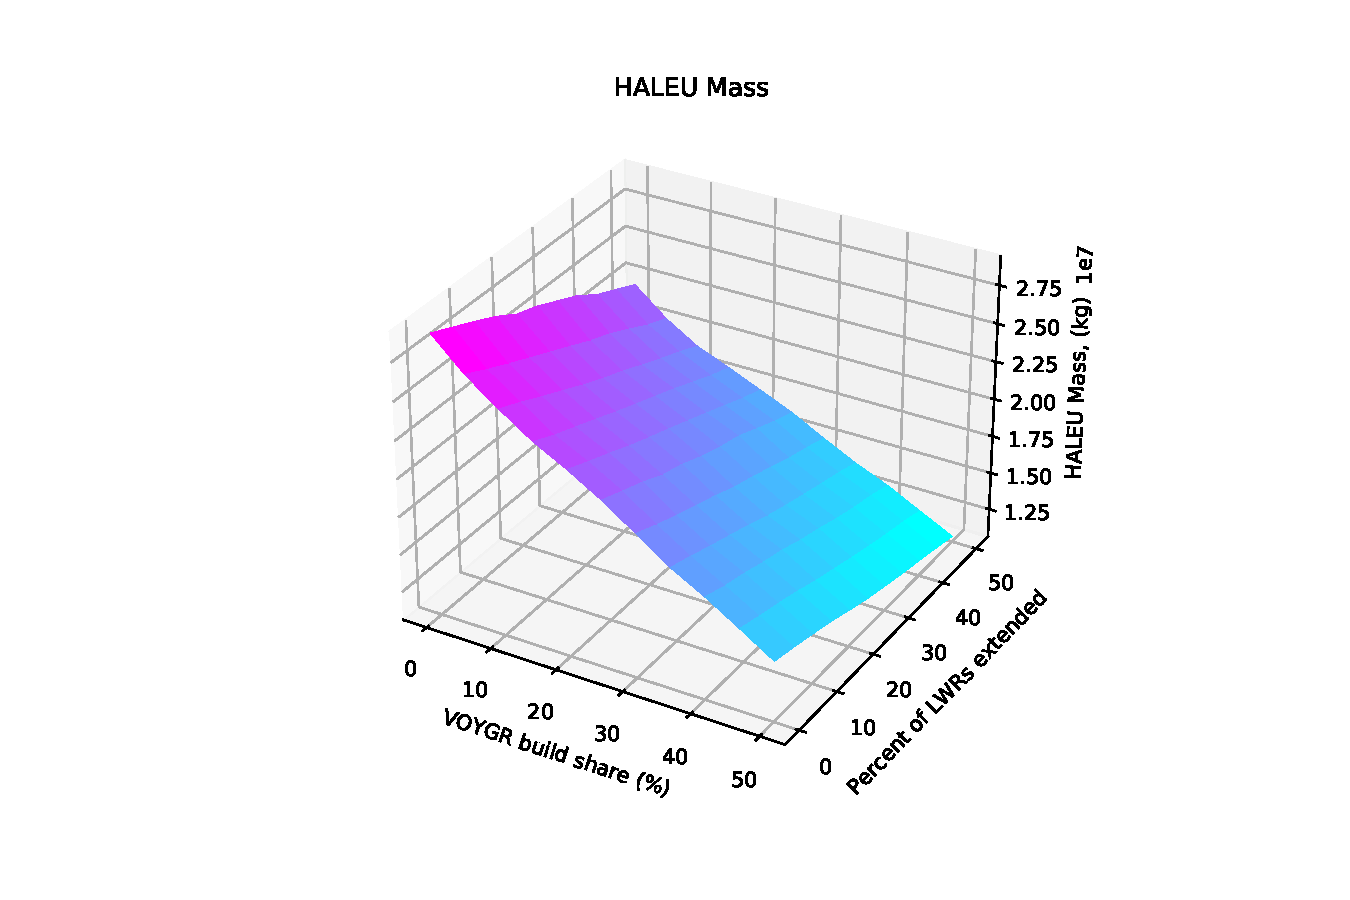
\includegraphics[scale=0.7,trim=120 0 120 30, clip]{lwr_voygr_share_haleu.pdf}
    \caption{Effect of the LWR lifetime and VOYGR build share on the HALEU mass.}
    \label{fig:lwr_voygr_share_haleu}
\end{figure}

The total enriched uranium mass decreases with increasing \gls{LWR} 
lifetimes, but increases with increasing VOYGR build share. There is a 
greater decrease in the total fuel mass required as the \gls{LWR} 
lifetime increases for greater values of VOYGR build share. 
\begin{figure}[ht]
    \centering
    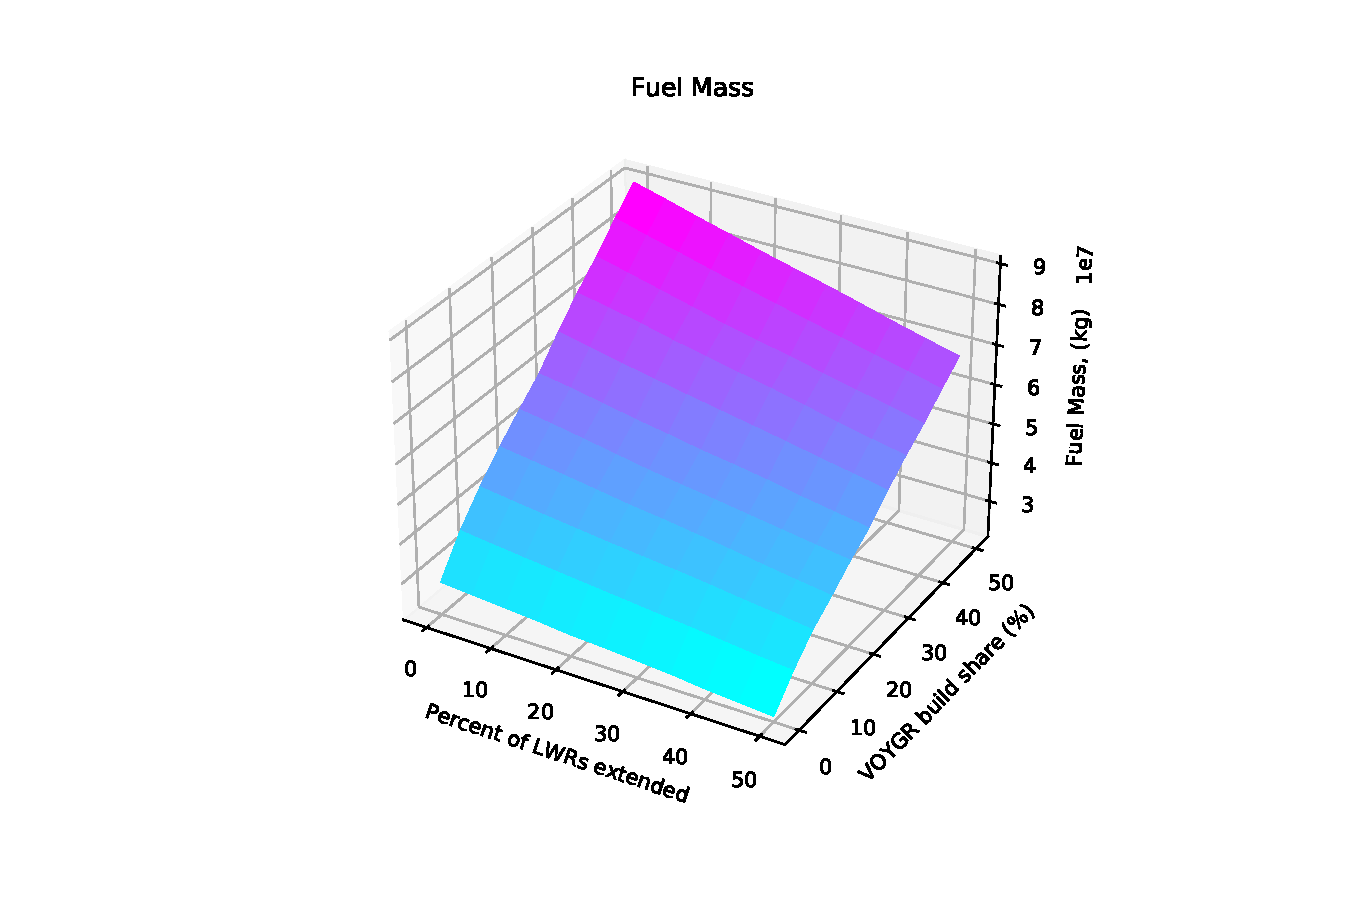
\includegraphics[scale=0.7,trim=120 0 120 30, clip]{lwr_voygr_share_enr_u.pdf}
    \caption{Effect of the LWR lifetime and VOYGR build share on 
    the total enriched uranium mass.}
    \label{fig:lwr_voygr_share_enr_u}
\end{figure}

\subsubsection{Xe-100 build share and Xe-100 burnup}
When the Xe-100 build share and discharge burnup are varied together
there is a strong combined effect on the metrics. The \gls{HALEU} 
mass required (figure \ref{fig:xe100_share_xe100_burnup_haleu}) 
increases as the burnup decreases and as the Xe-100 share increases.
The combined effect of these parameters is pronounced, such that there 
is a large increase in the \gls{HALEU} mass as the Xe-100 burnup 
reaches its minimum and the Xe-100 build share reaches its maximum. This 
results stems from a larger portion of the advanced reactor fleet 
using its fuel less efficiently as this corner of the input space is 
reached. This result suggests that the discharge burnup of an advanced 
reactor should be considered when determining the build share of a reactor
type, if this metric is important. 

\begin{figure}[h!]
    \centering
    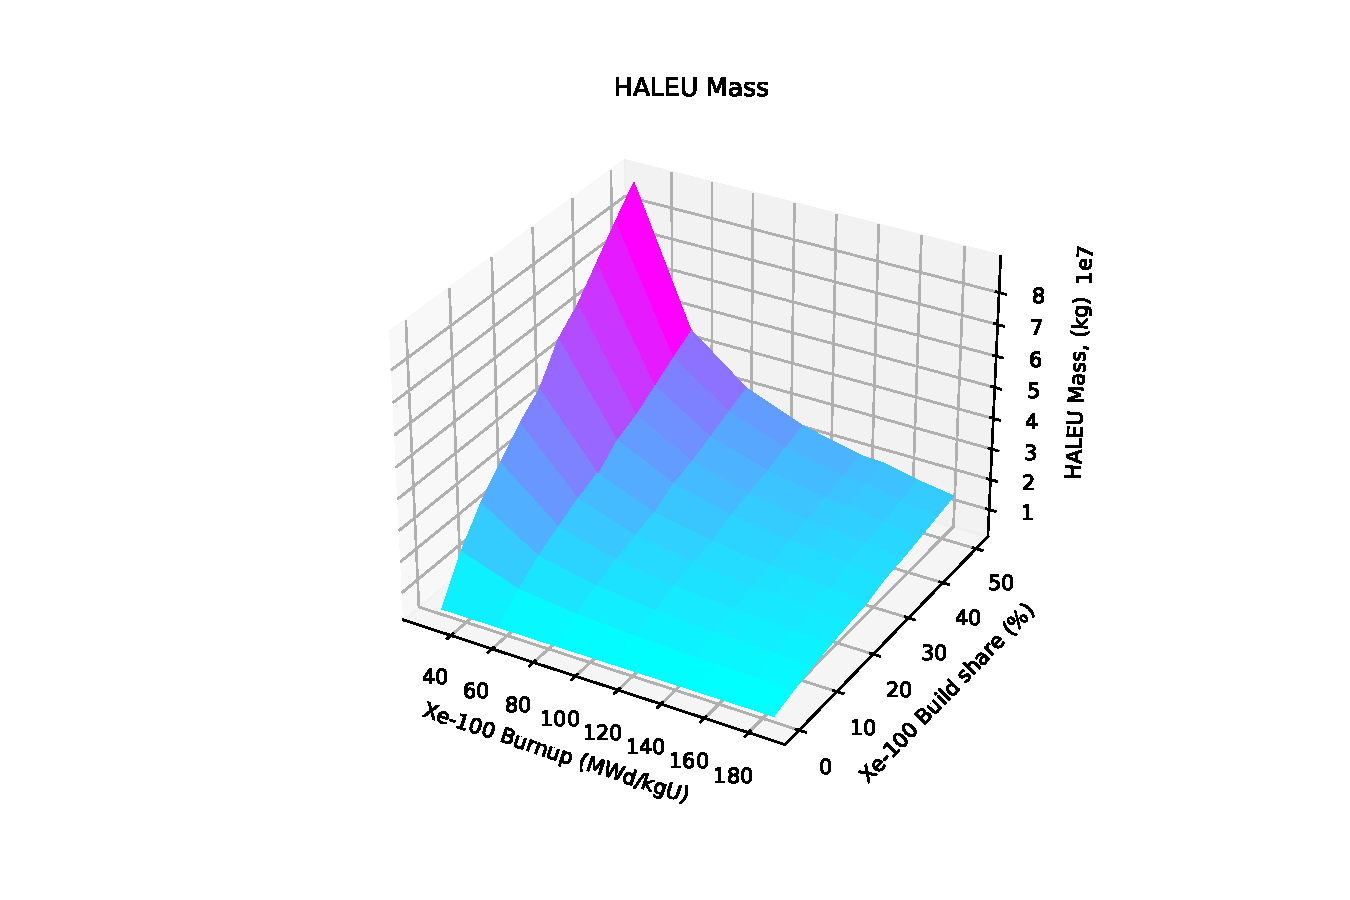
\includegraphics[scale=0.7, trim=120 0 120 30, clip]{xe100_share_xe100_burnup_haleu.pdf}
    \caption{Effect of Xe-100 discharge burnup and Xe-100 build share 
    on HALEU mass.}
    \label{fig:xe100_share_xe100_burnup_haleu}
\end{figure}

The total fuel mass reaches a minimum with a maximum Xe-100 build share 
and Xe-100 discharge burnup, which matches the trends observed in the 
\gls{OAT} analysis. A minimum is reach in this corner of the parameter 
space because more of the advanced reactor fleet is getting more 
energy out of the fuel used, so less fuel is required. Variations in the 
Xe-100 burnup do not affect the results when there is a 0\% Xe-100 build 
share because no Xe-100s are deployed. The Xe-100 build share does not 
greatly affect the fuel mass required when the Xe-100 has a discharge 
burnup of 28 MWd/kgU (the lowest value used in this work) because at this 
burnup level, the Xe-100 requires a similar amount of enriched uranium as 
the VOYGR for each 18 month period. Therefore, as the VOYGRs are replaced 
with Xe-100s as the Xe-100 build share increases the cumulative total 
fuel mass required does not change much. 

\begin{figure}[h!]
    \centering
    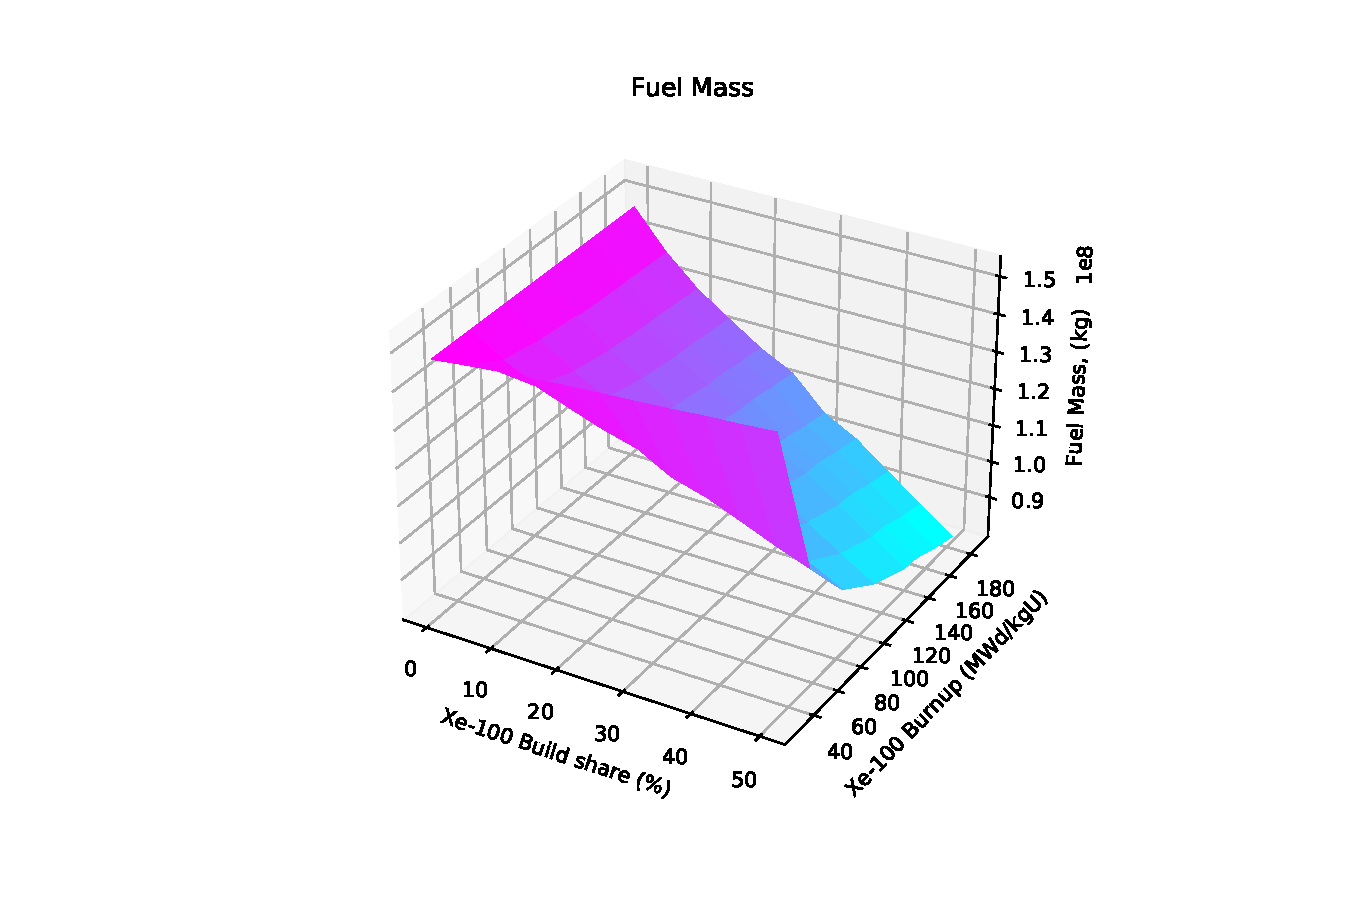
\includegraphics[scale=0.7, trim=120 0 120 30, clip]{xe100_share_xe100_burnup_enr_u.pdf}
    \caption{Effect of xe-100 discharge burnup and Xe-100 build share 
    on total fuel mass.}
    \label{fig:xe100_share_xe100_burnup_enr_u}
\end{figure}

\subsubsection{MMR build share and Xe-100 burnup}
When the \gls{MMR} build share and Xe-100 burnup are varied together, 
the effect on the metrics is not as consistent as the results from varying 
other pairs of parameters. As the Xe-100 burnup increases the fuel mass 
decreases. However, the effect of increasing the \gls{MMR} build share 
is dependent on the Xe-100 discharge burnup. At smaller Xe-100 discharge 
burnup values the fuel mass decreases with increasing \gls{MMR} build share. 
But at larger Xe-100 discharge burnup values the fuel mass increases 
with increasing \gls{MMR} build share. The different trends result from 
changes in how much fuel the Xe-100 requires at each refueling and 
the difference between that and the amount of fuel required by the \gls{MMR}.
At the lowest burnup values, the Xe-100 requires more fuel than the 
\gls{MMR}, so as more of the advanced reactor fleet is \glspl{MMR}, the 
total mass of fuel required in the transition decreases. However, as 
the Xe-100 burnup increases the Xe-100 requires less fuel than the 
\gls{MMR}. Therefore, requiring more of the advanced reactor fleet to be 
\glspl{MMR} increases the total fuel mass required by advanced reactors in 
the transition. This pattern of results is observed for all six metrics
considered in this work. 

\begin{figure}[h!]
    \centering
    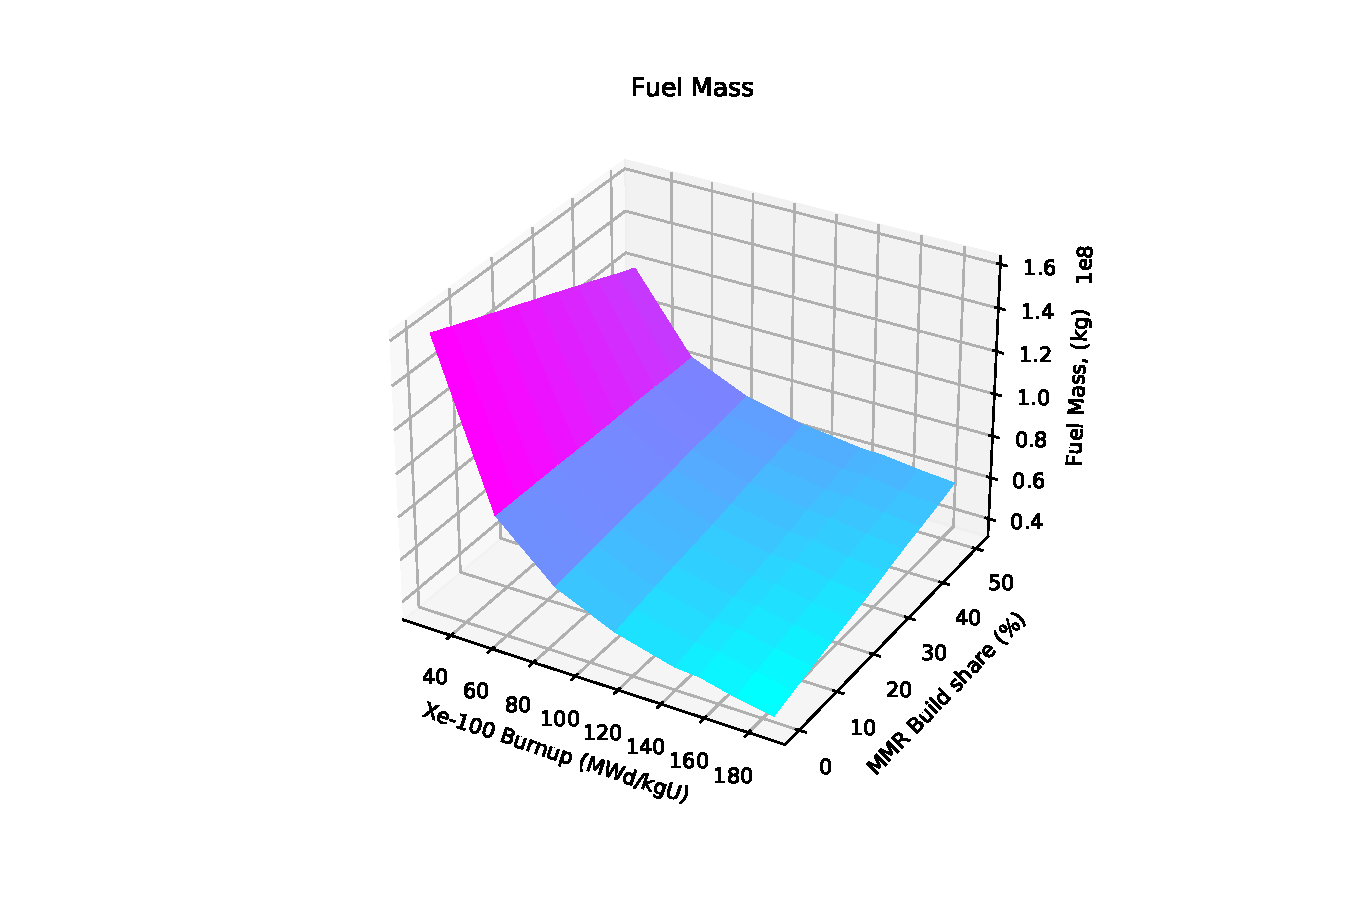
\includegraphics[scale=0.7, trim=120 0 120 30, clip]{mmr_share_xe100_burnup_enr_u.pdf}
    \caption{Effect of xe-100 discharge burnup and MMR build share 
    on total fuel mass.}
    \label{fig:mmr_share_xe100_burnup_enr_u}
\end{figure}


\subsubsection{Transition start and Xe-100 build share}
As Figure \ref{fig:ts_xe100_share_enr_u} shows, as the Xe-100 build 
share increases the total fuel mass decreases. However, there is little 
effect in the total fuel mass as the transition start time is delayed. This 
observation occurs because the magnitude of the effect on the fuel mass 
from varying the Xe-100 build share is greater than the magnitude of 
the effect from varying the transition start time. This is consistent 
with the results from the \gls{OAT} analysis, and is observed for five 
of the metrics considered in this work. This result suggests that the 
transition start time is not as important as the other parameters when 
trying to minimize or maximize certain metrics. 

\begin{figure}[h!]
    \centering
    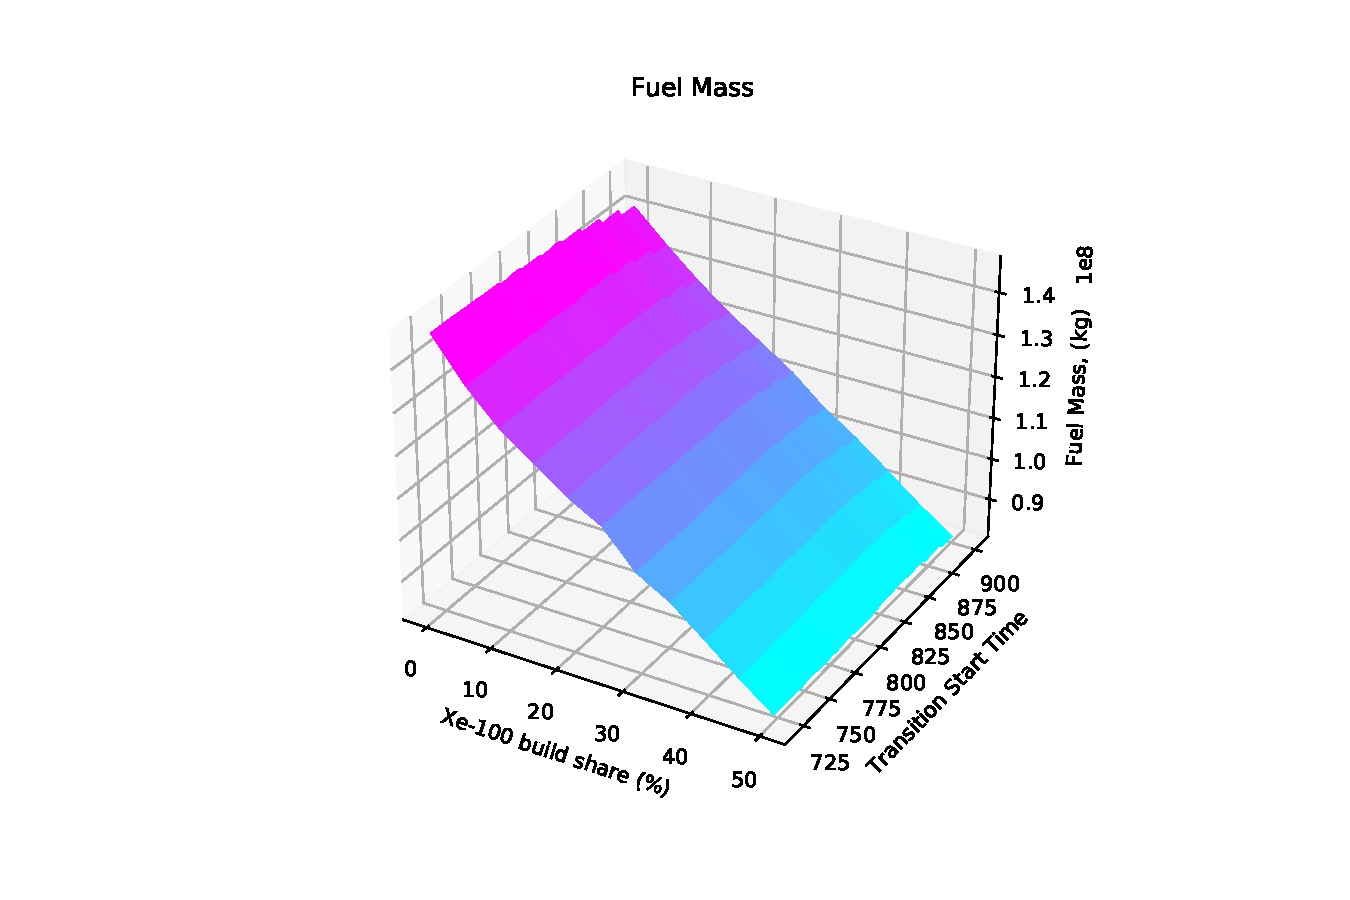
\includegraphics[scale=0.7, trim=120 0 120 0, clip]{ts_xe100_share_enr_u.pdf}
    \caption{Effect of transition start time and Xe-100 build share 
    on total fuel mass.}
    \label{fig:ts_xe100_share_enr_u}
\end{figure}

The effect of varying these two parameters is the opposite when the total 
\gls{SWU} capacity is considered: varying the transition start time has 
a greater impact on the metric than varying the Xe-100 build share. This 
result stems from the similar \gls{SWU} capacities needed for the Xe-100 
and VOYGR leading to little change in the total \gls{SWU} capacity when 
varying the Xe-100 build share. Therefore, the transition start time has 
more impact on this metric than the Xe-100 build share, and there is little 
of a combined effect observed because of the small impact from each parameter 
on this metric. 

\begin{figure}[h!]
    \centering
    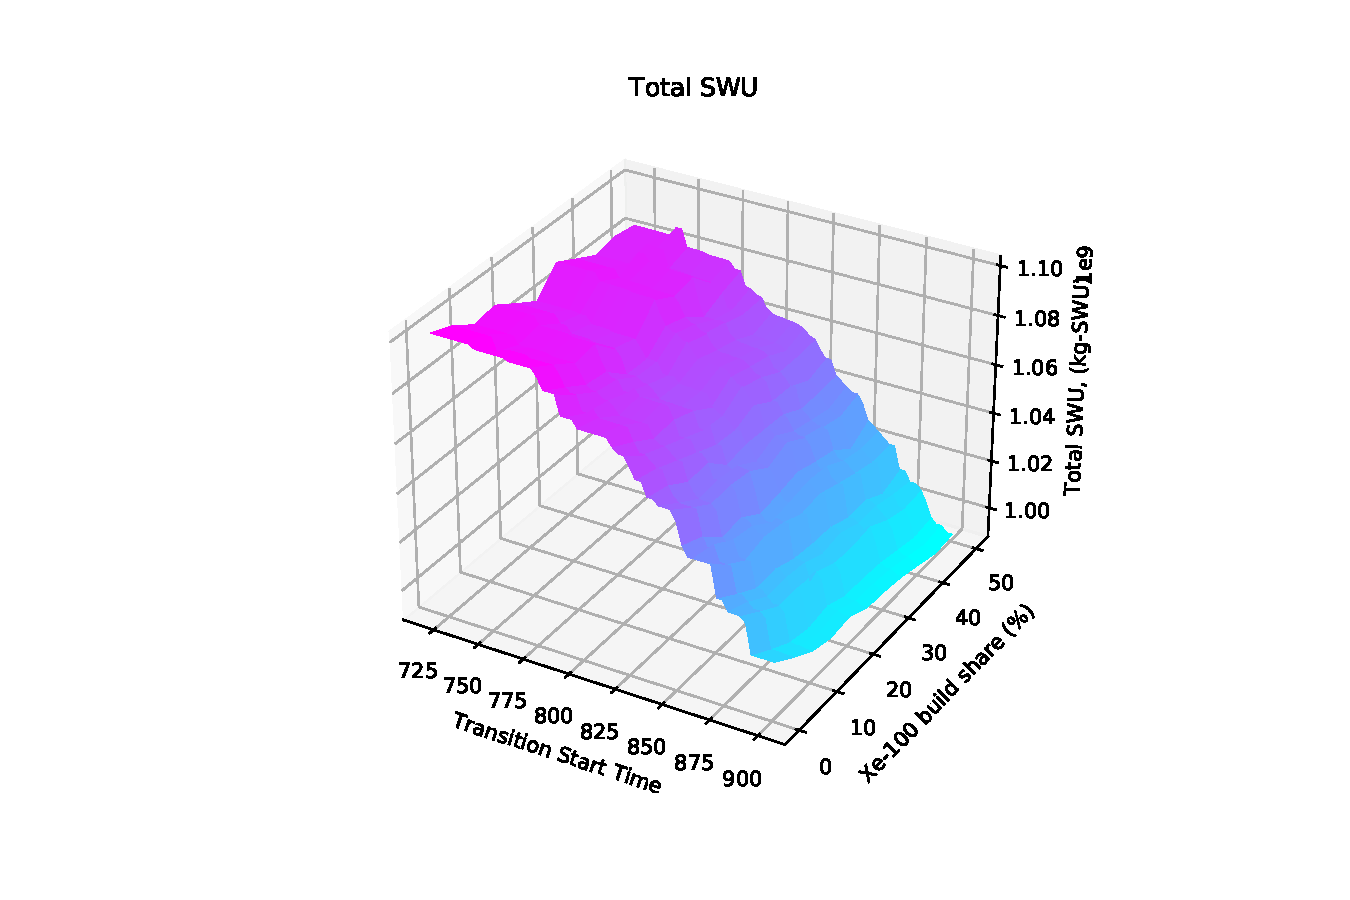
\includegraphics[scale=0.7, trim=120 0 120 0, clip]{ts_xe100_share_swu.pdf}
    \caption{Effect of transition start time and Xe-100 build share 
    on total fuel mass.}
    \label{fig:ts_xe100_share_swu}
\end{figure}

\subsection{Scenario 14}

\section{Global}
In each calculation of the global sensitivity analysis, the transition start 
time, percent of \glspl{LWR} operating for 80 years, the Xe-100 discharge 
burnup, \gls{MMR} burnup, and build share of one advanced reactor were 
varied. We decided to perform this analysis three separate times instead of 
varying all seven variables to prevent unwanted combinations of the 
advanced reactor build shares that result in large oversupplies or 
undersupplies of power. 

All of the variables included in this work can physically take any non-negative 
real value. However, the discharge burnup values used in this work are specific 
integer values. To reconcile the use of specific values when others are physical, 
we created surrogate models, similar to the ones used by Richards and Feng 
\cite{richards_application_2021}. We generated the data for the model by sampling 
across the input space 4500 times because the Dakota user's manual 
\cite{adams_dakota_2019} suggests running 

\begin{equation}
    100\times P\times(R+2)
\end{equation}

in which $P$ is the number of input parameters and $R$ is the number out response 
metrics. To assist in creation of the surrogate model, the \gls{MMR} burnup 
was converted from a discrete variable to a continuous variable by varying 
the lifetime of the reactor as need to achieve the burnup value. The 
\gls{MMR} burnup was restricted to between 41-90 MWd/kgU, the range 
for the values used in the other sensitivity analysis. 
The Xe-100 discharge burnup values were expanded as well, but remained 
a discrete variable. Additional burnup points were selected to represent 
between one and six passes for each pebble with a residence time of six, seven, 
or eight months for each pass. This expansion of the Xe-100 burnup resulted 
in 16 different burnup values between 28-185 MWd/kgU. The other variables were 
only restricted to the specified range previously used for the variable (e.g., 
0-50\% for the \gls{LWR} lifetime extensions) and were treated as continuous 
variables.
We randomly sampled (using the Latin Hypercube Sampling 
method in Dakota) each continuous variable based on the possible values and 
calculated the metrics for these samples. This data was then used to create 
the surrogate model to perform the global sensitivity analysis and 
calculate the Sobol' indices. 

When creating the surrogate model we once again used random sampling for all 
of the variables, but allowed all of the input parameters to be continuous 
variables. 
We used both the gaussian and quadratic fits to the data 
to create the surrogate models, similar to what Richards and 
Feng did \cite{richards_application_2021}. 
We also instructed Dakota to perform variance decomposition 
on the surrogate model so that Sobol' indices would be calculated. The 
results presented in this section are the Sobol' indices that describes the 
impact of each input parameter on each output metric. The total and the main 
Sobol' indices are reported, which describe the contribution from the parameter 
and its interactions with all of the other parameters and the contribution from 
just the parameter, respectively. 

\subsection{Scenario 7}

\subsubsection{Xe-100 build share}
When running the gaussian surrogate model for the variations in the Xe-100 build 
share, the models all  have an R$^2$ value of 1, which means that the outputs of 
the surrogate models match perfectly to the data provided from the initial 
\Cyclus runs. The large R$^2$ value suggests that this surrogate model type 
fits to noise in the data provided. A comparison of the results of the 
gaussian surrogate model and the data provided to the model shows some interesting 
results. Figure \ref{fig:s7_xe100_gaussian} compares the values of the
\gls{HALEU} mass as a function of the Xe-100 burnup for the Gaussian model 
and the input data. The results of the Gaussian model follows the input 
data well, nearly reaching the maximum and minimums of the data. However, 
closer inspection of the data shows that results of the Gaussian model 
include non-physical results, such as negative values of \gls{HALEU} mass. 
These values suggest that the Gaussian model is extrapolating some, instead 
of just interpolating. Therefore, the Gaussian model is not a perfect 
match to the input data, which means that the Sobol' indices are different 
than if the variance decomposition were performed on the input data. 

\begin{figure}
    \centering 
    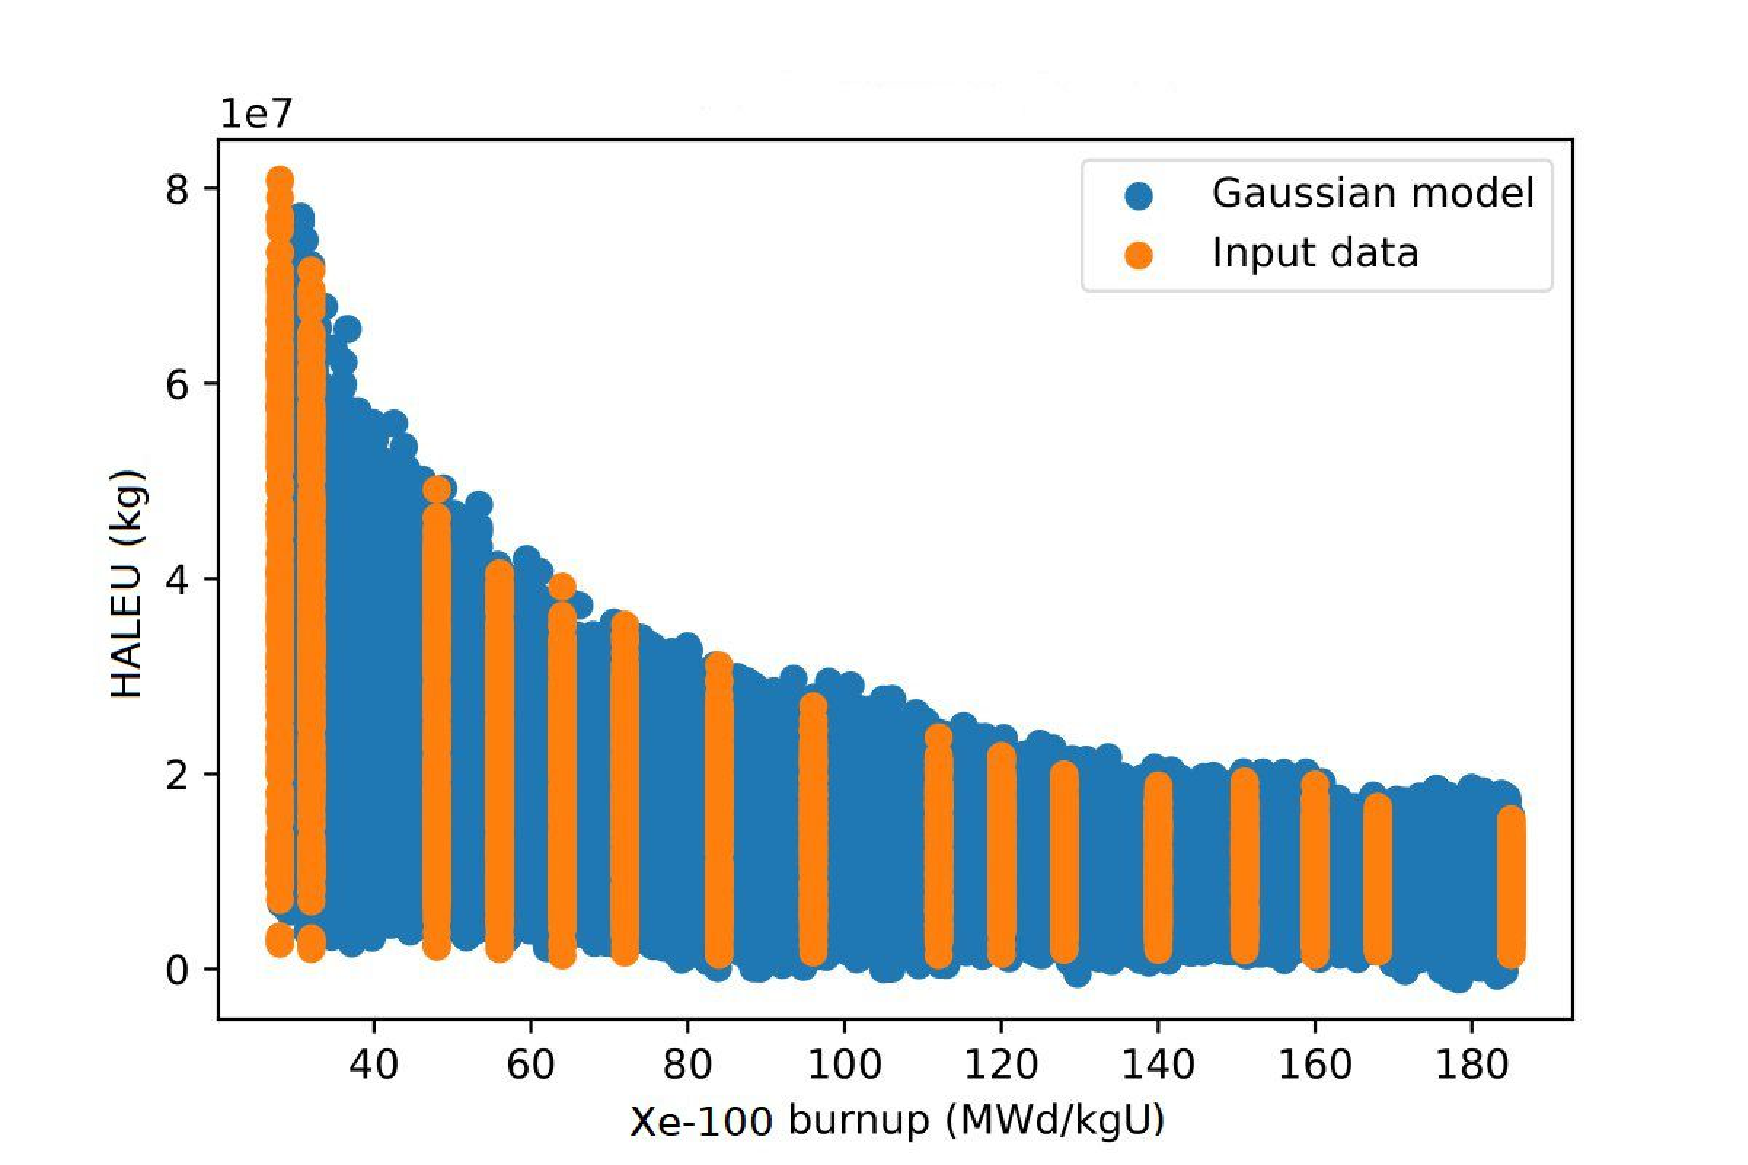
\includegraphics[scale=0.8]{xe100_share_gaussian_xe100_burnup_haleu.pdf}
    \caption{Comparison of the input data and the results of the gaussian 
    surrogate model when the Xe-100 build share is varied. }
    \label{fig:s7_xe100_gaussian}
\end{figure}

Table \ref{tab:s7_sobol_xe100_gaussian} reports the main and total Sobol' indices 
for each input parameter on each output metric. The highlighted cells have 
a total Sobol' index of at least 0.5. The Xe-100 build share and Xe-100 
burnup have the largest Sobol' indices for most of the output metrics. 

The \gls{MMR} burnup has a small Sobol' index for all of the output metrics
because a very small portion of the fleet are \glspl{MMR}. The Xe-100 build share 
does not have as much of an impact on the total \gls{SWU} capacity, compared 
with its impact on the other metrics, because of the similar \gls{SWU} 
capacity required by the Xe-100 and the VOYGR, and the replacement of Xe-100s 
with VOYGRs as the Xe-100 build share decreases. The transition start time 
has little effect on any of the metrics, which is consistent with the 
results of the \gls{OAT} and synergistic analysis. The \gls{LWR} lifetimes 
do not greatly affect any of the \gls{HALEU}-related metrics or the 
total \gls{SWU} capacity. This parameter has some impact on the total 
fuel mass and the \gls{SNF} mass, but less of an impact than the Xe-100 
build share. 

The Xe-100 build share has the largest impact on the \gls{SNF} mass, and 
the other parameters do not have much of an impact. This parameter 
has more of an impact on the \gls{SNF} mass than the other parameters because 
of the replacement of Xe-100s with VOYGRs as the Xe-100 build share decreases. 
The VOYGR 

\begin{table}
    \centering
    \caption{Sobol' indices for the Gaussian model when varying the 
    Xe-100 build share. The first value is the 
    main index, the second value is the total index.}
    \label{tab:s7_sobol_xe100_gaussian}
    \begin{tabular}{c c c c c c c}
        \hline
        & \multicolumn{6}{c}{Output Metric} \\
        Parameter & Fuel Mass & HALEU Mass & SWU & HALEU SWU & Feed & SNF Mass \\
        \hline
        Transition Start & 0.003/0.003 & 0.007/0.007 & 0.007/0.009 &
                           0.009/0.009 & 0.006/0.009 & 0.003/0.003\\
        LWR Lifetime & 0.268/0.280 & 0.012/0.021 & 0.081/0.095 &
                       0.013/0.022 & 0.013/0.022 & 0.301/0.314\\
        Xe-100 Build Share & \cellcolor{green!25}0.478/0.533 & \cellcolor{green!25}0.375/0.513 & 0.099/0.283 &
        \cellcolor{green!25}0.374/0.511 & \cellcolor{green!25}0.374/0.512 & 0.411/0.474\\
        Xe-100 Burnup & 0.188/0.247 & \cellcolor{green!25}0.465/0.571 & \cellcolor{green!25}0.622/0.775 & 
        \cellcolor{green!25}0.463/0.568 & \cellcolor{green!25}0.463/0.568 & 0.214/0.280\\
        MMR Burnup & 0.002/0.002 & 0.003/0.004 & 0.005/0.006 & 
                     0.004/0.005 & 0.004/0.005 & 0.002/0.002\\
        \hline        
    \end{tabular}
\end{table}

When using a quadratic surrogate model, the R$^2$ values for the training points on 
each output metric range between 0.921-0.966. Therefore, these model are still expected to 
fit the input data provided but not be fit to the noise in the input data 
as much as the Gaussian models. A comparison of the Xe-100 burnup and \gls{HALEU} 
mass for the input data and the results of the quadratic model (Figure 
\ref{fig:s7_xe100_quadratic}) shows that the quadratic model does 
capture the overall trend of the input data. However, like the Gaussian model, 
the quadratic model gives the non-physical result of a negative mass. Additionally, 
the results of the quadratic model do not meet the maximum of the input data and 
provide multiple results below the minimum value of the input data. Therefore, 
the quadratic model is also performing some extrapolation of the data based on the 
fit placed on the data.

\begin{figure}
    \centering 
    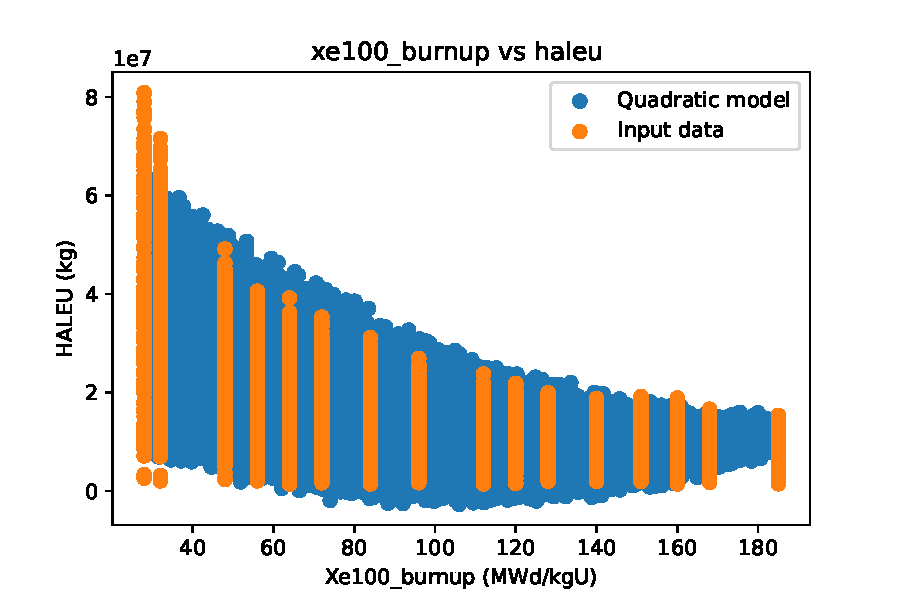
\includegraphics[scale=0.8]{xe100_share_quadratic_xe100_burnup_haleu.pdf}
    \caption{Comparison of the input data and the results of the gaussian 
    surrogate model when the Xe-100 build share is varied.}
    \label{fig:s7_xe100_quadratic}
\end{figure}

The Sobol' indices for each input parameter on each metric from the quadratic 
surrogate model are shown in Table \ref{tab:s7_sobol_xe100_quadratic}. The 
green cells identify total Sobol' indices that are at least 0.5. The same patterns 
observed in the Sobol' indices from the Gaussian model are 
observed in the values from the quadratic model as well. The Xe-100 build share 
and Xe-100 burnup affect the metrics the most, the \gls{LWR} lifetime has some 
impact, and the \gls{MMR} burnup and transition start time has the smallest impact 
on the metrics. 

\begin{table}
    \centering
    \caption{Sobol' indices for the quadratic model when varying the Xe-100 
    build share. The first number is the main index, the second is the total 
    index.}
    \label{tab:s7_sobol_xe100_quadratic}
    \begin{tabular}{c c c c c c c}
        \hline
        & \multicolumn{6}{c}{Output Metric} \\
        Parameter & Fuel Mass & HALEU Mass & SWU & HALEU SWU & Feed & SNF Mass \\
        \hline
        Transition Start & 0.000/0.000& 0.006/0.005 & 0.007/0.007 &
                           0.008/0.007 & 0.008/0.007 & 0.002/0.004\\
        LWR Lifetime & 0.278/0.286 & 0.014/0.021 & 0.082/0.089 & 
                       0.015/0.022 & 0.015/0.022 & 0.310/0.319\\
        Xe-100 Build Share & \cellcolor{green!25}0.443/0.501 & \cellcolor{green!25}0.374/0.500 & 0.115/0.283 & 
                             0.374/0.499 & 0.374/0.499 & 0.375/0.441\\
        Xe-100 Burnup & 0.214/0.279 & \cellcolor{green!25}0.472/0.578 & \cellcolor{green!25}0.624/0.773 &
                        \cellcolor{green!25}0.470/0.576 & \cellcolor{green!25}0.430/0.576 & 0.243/0.315\\
        MMR Burnup & 0.001/0.001 & 0.002/0.002 & 0.004/0.004 &
                     0.003/0.003 & 0.003/0.003 & 0.001/0.001\\
        \hline        
    \end{tabular}
\end{table}

Based on the results from each model, the Xe-100 build share and Xe-100 burnup 
should be varied to have the largest impact on the metrics

\subsubsection{MMR build share}
The Gaussian model has an R$^2$ value of 1 with respect to each of the output 
metrics. This value means that these models are also expected to fit the input 
data very well, including any noise present in the data. As Figure 
\ref{fig:s7_mmr_gaussian} shows, the data from the Gaussian model fits well 
to the input data provided. Unlike the models predicted based on input data when 
the Xe-100 build share was varied, this model does not result in any negative 
mass values. However, it still results in mass values lower than what is 
present in the input data which suggests that this model also extrapolates 
on some of the data. 

\begin{figure}
    \centering 
    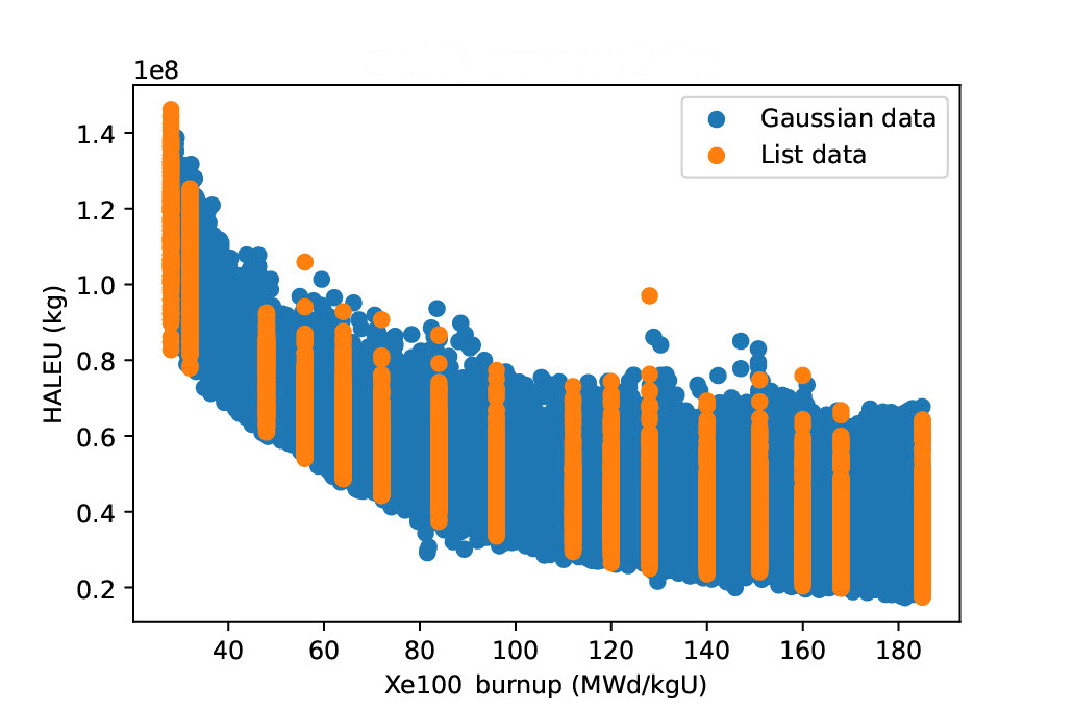
\includegraphics[scale=0.8]{mmr_share_gaussian_xe100_burnup_haleu.pdf}
    \caption{Comparison of the input data and the results of the Gaussian 
    surrogate model when the MMR build share is varied.}
    \label{fig:s7_mmr_gaussian}
\end{figure}

Examination of the Sobol' indices for this model (Table \ref{tab:s7_sobol_mmr_gaussian})
shows that the Xe-100 burnup has the largest impact on all of the 
output metrics. This is somewhat surprising, as one may expect the \gls{MMR} 
build share and \gls{MMR} burnup to have a strong combined impact on 
the results. However, this result is consistent with the results 
shown for the synergistic analysis (Figures \ref{fig:mmr_share_xe100_burnup} and 
\ref{fig:mmr_share_mmr_burnup}). When the Xe-100 burnup was varied on combination 
with the \gls{MMR} share, the range of values for each metric was larger than 
when the \gls{MMR} burnup was varied with the \gls{MMR} build share. 

Similar to the results from varying the Xe-100  build share, the 
transition start time has no impact on the results. The \gls{LWR} 
lifetime has less of an impact on the metrics than when the Xe-100 
build share was varied. The \gls{MMR} has almost no impact on the 
output metrics. 

\begin{table}
    \centering
    \caption{Sobol' indices for the Gaussian model when varying the MMR 
    build share. The first number is the main index, the second is the total 
    index.}
    \label{tab:s7_sobol_mmr_gaussian}
    \begin{tabular}{c c c c c c c}
        \hline
        & \multicolumn{6}{c}{Output Metric} \\
        Parameter & Fuel Mass & HALEU Mass & SWU & HALEU SWU & Feed & SNF Mass \\
        \hline
        Transition Start & 0.001/0.006 & 0.000/0.004 & 0.001/0.001 &
                           0.001/0.001 & 0.001/0.001 & 0.001/0.006\\
        LWR Lifetime & 0.054/0.068 & 0.047/0.063 & 0.055/0.071 &
                       0.054/0.069 & 0.054/0.069 & 0.057/0.071\\
        MMR Build Share & 0.069/0.107 & 0.068/0.107 & 0.162/0.203 &
                          0.162/0.204 & 0.152/0.193 & 0.015/0.055\\
        Xe-100 Burnup & \cellcolor{green!25}0.806/0.846 & \cellcolor{green!25}0.819/0.858 & \cellcolor{green!25}0.700/0.732 &
        \cellcolor{green!25}0.701/0.734 & \cellcolor{green!25}0.713/0.747 & \cellcolor{green!25}0.858/0.900\\
        MMR Burnup & 0.035/0.049 & 0.037/0.050 & 0.054/0.071 &
                     0.054/0.071 & 0.052/0.069 & 0.038/0.053\\
        \hline        
    \end{tabular}
\end{table}

When using the quadratic surrogate model, the models have R$^2$ values of 0.94
with respect to each of the output metrics. Therefore, these models also fit 
the data well without fitting all of the noise present in the input data. 
As Figure \ref{fig:s7_mmr_quadratic} shows, the output of the quadratic model 
fits the input data well, but not perfectly. Similar to the quadratic 
model created from varying the Xe-100 build share, this model 
does not perform well in fitting the maximum values and under-predicts 
some of the minimum values in the input data. 

\begin{figure}
    \centering 
    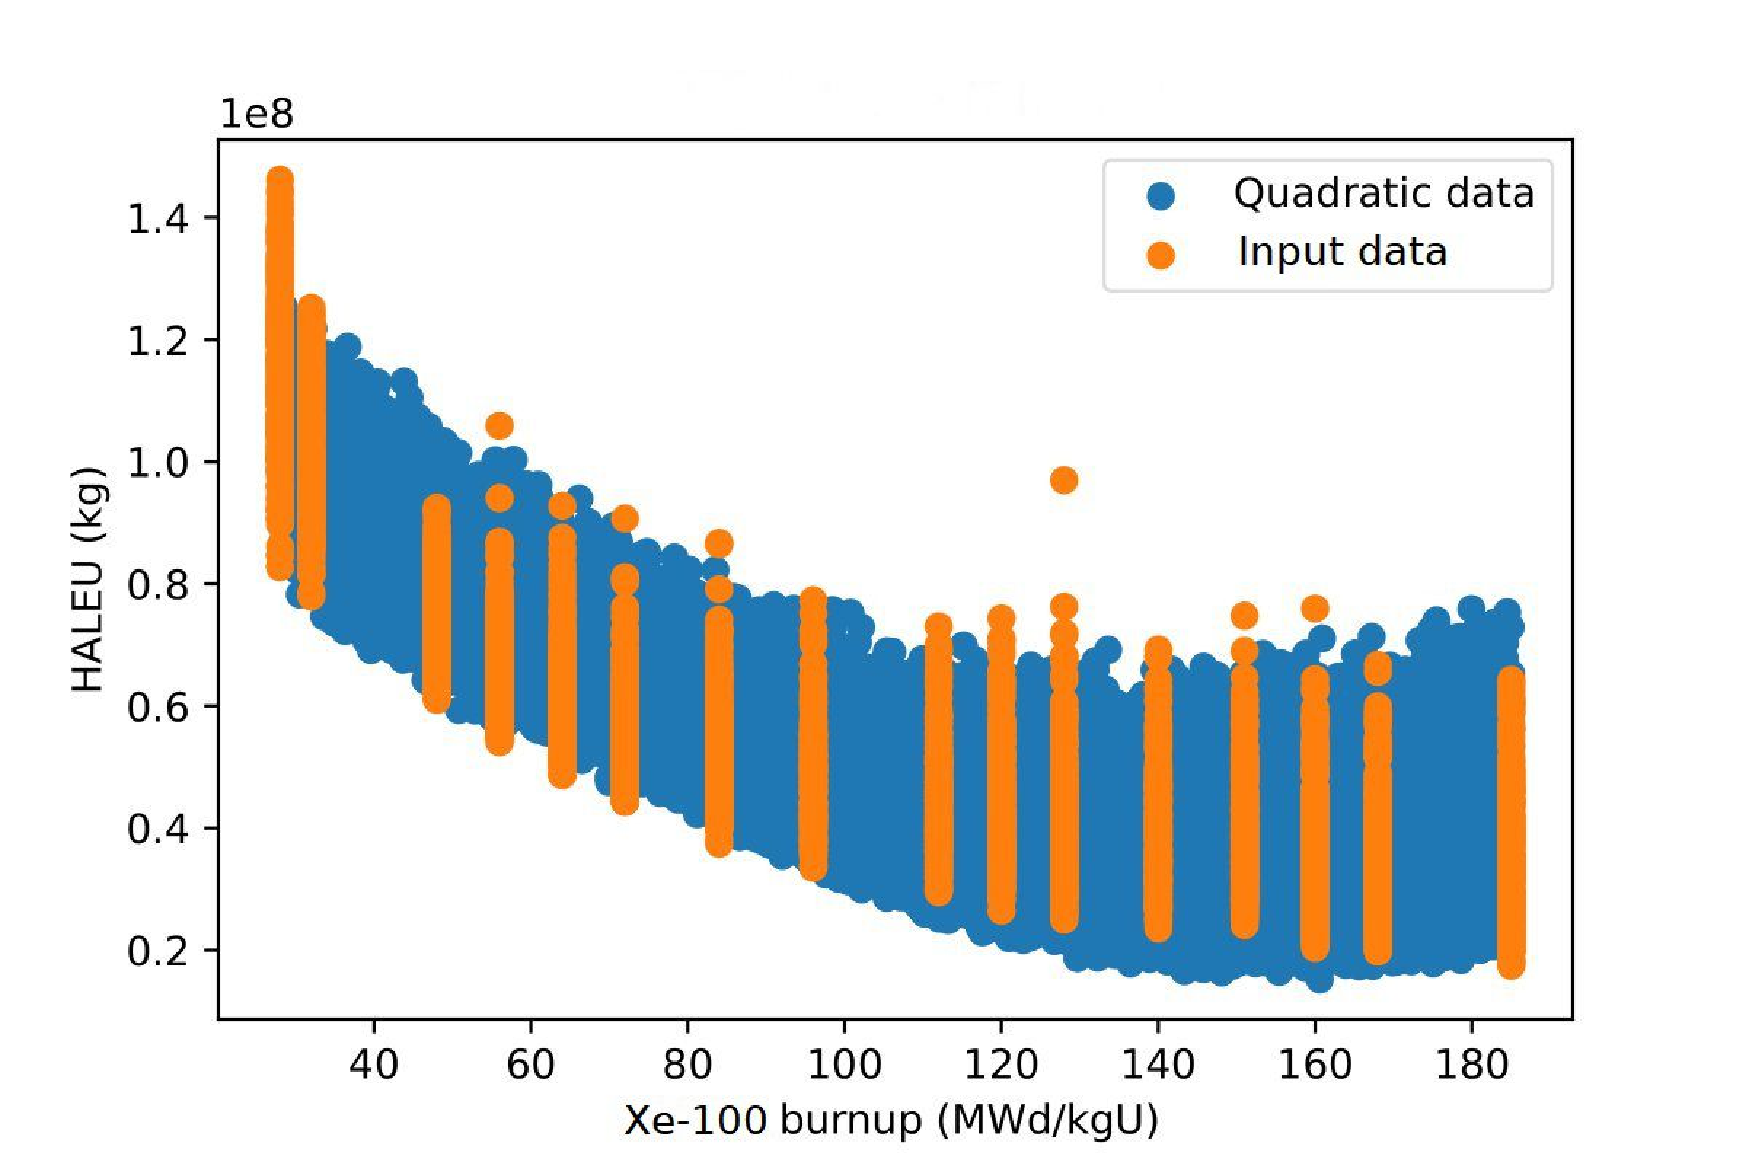
\includegraphics[scale=0.8]{mmr_share_quadratic_xe100_burnup_haleu.pdf}
    \caption{Comparison of the input data and the results of the quadratic 
    surrogate model when the MMR build share is varied.}
    \label{fig:s7_mmr_quadratic}
\end{figure}

The Sobol' indices from the quadratic model are similar to those from the 
Gaussian model. The Xe-100 burnup has the largest impact on all of the 
output metrics. The \gls{MMR} build share has the next largest impact 
on the metrics, but it is a very small impact. The other model 
parameters have a negligible effect on the metrics. 

\begin{table}
    \centering
    \caption{Sobol' indices for the quadratic model when varying the MMR 
    build share. The first number is the main index, the second is the total 
    index.}
    \label{tab:s7_sobol_mmr_quadratic}
    \begin{tabular}{c c c c c c c}
        \hline
        & \multicolumn{6}{c}{Output Metric} \\
        Parameter & Fuel Mass & HALEU Mass & SWU & HALEU SWU & Feed & SNF Mass \\
        \hline
        Transition Start & 0.002/0.003 & 0.000/0.000 & 0.000/0.000 &
                        0.000/0.000 & 0.000/0.000 & 0.002/0.003\\
        LWR Lifetime & 0.023/0.062 & 0.046/0.054 & 0.050/0.059 &
                       0.049/0.057 & 0.049/0.057 & 0.054/0.064\\
        MMR Build Share & 0.051/0.087 & 0.052/0.089 & 0.133/0.171 &
                          0.133/0.171 & 0.124/0.162 & 0.008/0.046\\
        Xe-100 Burnup & \cellcolor{green!25}0.834/0.866 & \cellcolor{green!25}0.846/0.875 & \cellcolor{green!25}0.742/0.764 &
        \cellcolor{green!25}0.742/0.765 & \cellcolor{green!25}0.753/0.777 & \cellcolor{green!25}0.879/0.909\\
        MMR Burnup & 0.034/0.039 & 0.034/0.040 & 0.050/0.058 & 
                     0.050/0.058 & 0.048/0.056 & 0.035/0.041\\
        \hline        
    \end{tabular}
\end{table}

The results of these models emphasize the role that the Xe-100 burnup 
plays in the material requirements of these fuel cycles. 

\subsubsection{VOYGR build share}
The R$^2$ values for the Gaussian model with respect to 
each output metric is 1, similar to each of the other Gaussian 
models. Comparing the input data and the Gaussian model data 
(Figure \ref{fig:s7_voygr_gaussian}) shows that the data from the 
Gaussian model fits very well to the input data provided. 

\begin{figure}
    \centering 
    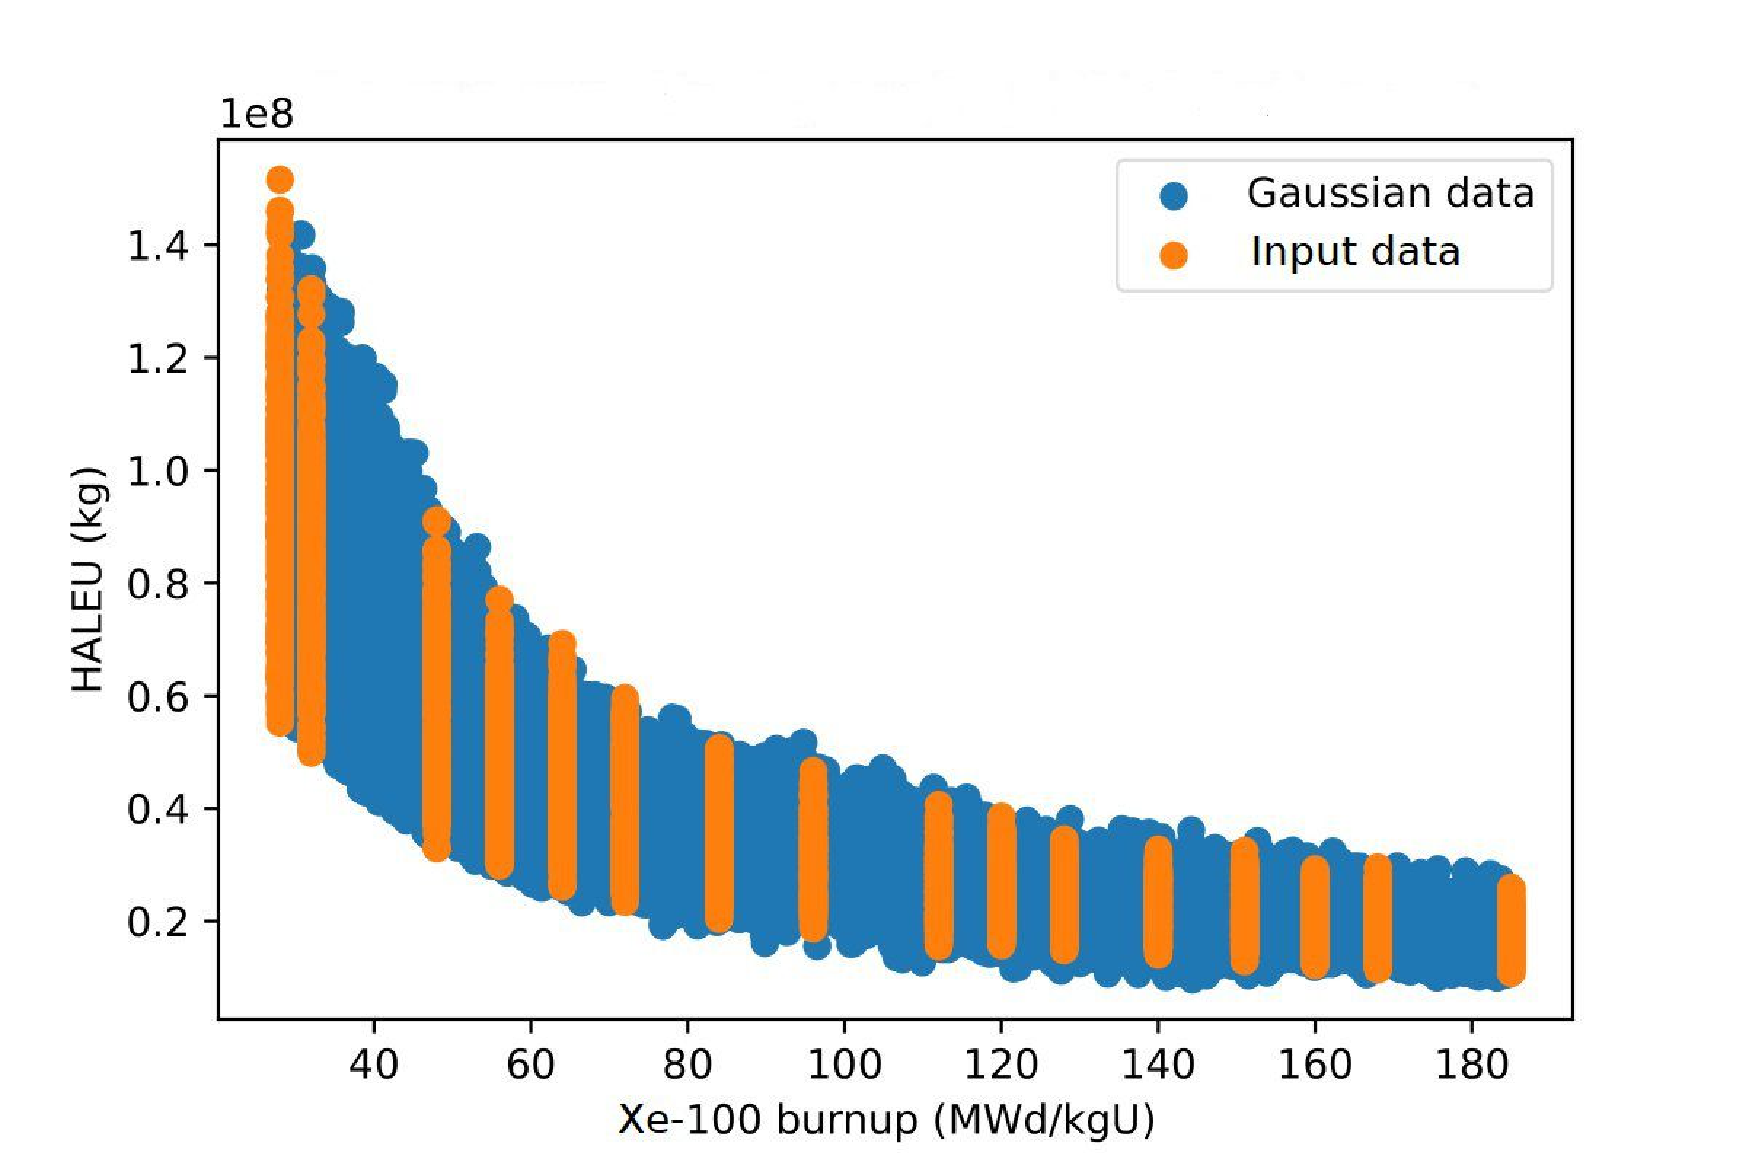
\includegraphics[scale=0.8]{voygr_share_gaussian_xe100_burnup_haleu.pdf}
    \caption{Comparison of the input data and the results of the Gaussian 
    surrogate model when the VOYGR build share is varied.}
    \label{fig:s7_voygr_gaussian}
\end{figure}

The Sobol' indices from this model, shown in Table \ref{tab:s7_sobol_voygr_gaussian}
show a similar trend to the Sobol' indices from varying the \gls{MMR}
build share. The Xe-100 burnup has the largest impact on all of the 
results, the transition start time and \gls{MMR} burnup have no 
effect on the metrics, and the \gls{LWR} lifetimes and VOYGR build share 
have a very small impact on the metrics. 

Based on the results of 
the \gls{OAT} analysis, increasing the VOYGR build share replaces 
Xe-100s with VOYGRs. Therefore, the VOYGR build share implicitly 
impacts the Xe-100 build share, which leads to this input parameter 
having a larger impact on the metrics than most of the other variables. 
The VOYGR build share has a larger impact on the fuel mass and the 
\gls{SNF} mass than the other metrics because the VOYGR takes in more 
and discharges more 
fuel than the Xe-100 and \gls{MMR} per unit time and energy. The 
increased impact of the VOYGR build share on these metrics leads to 
the decreased impact of the Xe-100 burnup, relative to the 
\gls{HALEU}-related metrics. 

\begin{table}
    \centering
    \caption{Sobol' indices for the Gaussian model when varying the VOYGR 
    build share. The first number is the main index, the second is the total 
    index.}
    \label{tab:s7_sobol_voygr_gaussian}
    \begin{tabular}{c c c c c c c}
        \hline
        & \multicolumn{6}{c}{Output Metric} \\
        Parameter & Fuel Mass & HALEU Mass & SWU & HALEU SWU & Feed & SNF Mass \\
        \hline
        Transition Start & 0.002/0.003 & 0.000/0.001 & 0.000/0.002 & 
                           0.000/0.001 & 0.000/0.001 & 0.001/0.003\\
        LWR Lifetime & 0.065/0.076 & 0.020/0.033 & 0.033/0.045 & 
                       0.020/0.033 & 0.020/0.033 & 0.069/0.081\\
        VOYGR Build Share & 0.252/0.284 & 0.114/0.0151 & 0.028/0.067 &
                            0.114/0.151 & 0.114/0.151 & 0.204/0.238\\
        Xe-100 Burnup & \cellcolor{green!25}0.652/0.683 & \cellcolor{green!25}0.837/0.883 & \cellcolor{green!25}0.910/0.956 & 
        \cellcolor{green!25}0.836/0.881 & \cellcolor{green!25}0.836/0.881 & \cellcolor{green!25}0.696/0.730\\
        MMR Burnup & 0.002/0.002 & 0.000/0.002 & 0.001/0.001 & 
                     0.001/0.002 & 0.001/0.002 & 0.002/0.002\\
        \hline        
    \end{tabular}
\end{table}

When using the quadratic fit, the R$^2$ values range between 0.94-0.95. 
These values are consistent with the R$^2$ values for the other 
quadratic models in this work. The data from this quadratic model,
compared with the input data in Figure \ref{fig:s7_voygr_quadratic}, 
shows that it does not fully reach the maximum of the input data
and under-predicts some of the minimum values. These trends have 
been observed in all of the quadratic models created for this analysis. 

\begin{figure}
    \centering 
    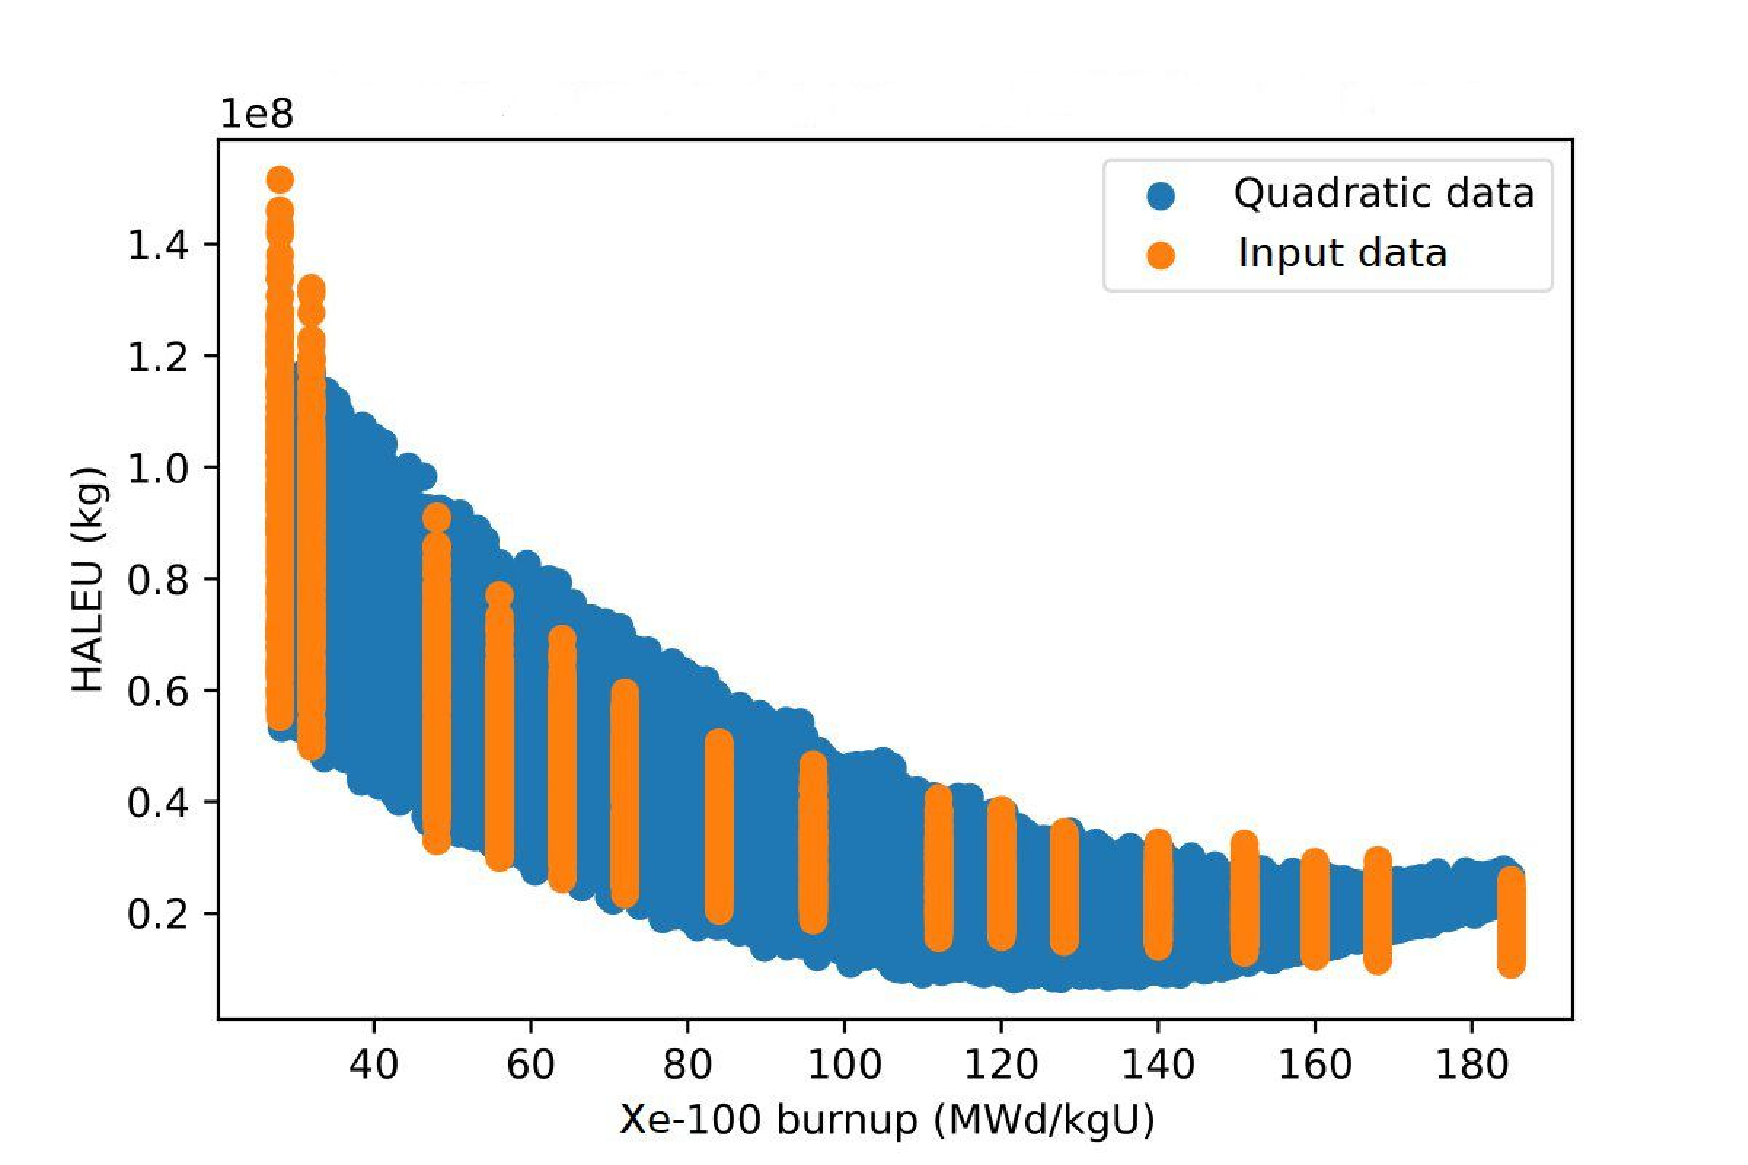
\includegraphics[scale=0.8]{voygr_share_quadratic_xe100_burnup_haleu.pdf}
    \caption{Comparison of the input data and the results of the quadratic 
    surrogate model when the VOYGR build share is varied.}
    \label{fig:s7_voygr_quadratic}
\end{figure}

The Sobol' indices from this model, given in Table \ref{tab:s7_sobol_voygr_quadratic},
have the same pattern as the Sobol' indices from the Gaussian model created. 
This data does not provide any new insights into how each input parameter
affects the output metrics of this transition scenario. 

\begin{table}
    \centering
    \caption{Sobol' indices for the quadratic model when varying the VOYGR 
    build share. The first number is the main index, the second is the total 
    index.}
    \label{tab:s7_sobol_voygr_quadratic}
    \begin{tabular}{c c c c c c c}
        \hline
        & \multicolumn{6}{c}{Output Metric} \\
        Parameter & Fuel Mass & HALEU Mass & SWU & HALEU SWU & Feed & SNF Mass \\
        \hline
        Transition Start & 0.002/0.002 & 0.000/0.000 & 0.000/0.001 &
                           0.000/0.000 & 0.000/0.000 & 0.001/0.002\\
        LWR Lifetime & 0.063/0.071 & 0.020/0.031 & 0.031/0.042 &
                       0.051/0.031 & 0.020/0.031 & 0.066/0.075\\
        VOYGR Build Share & 0.214/0.243 & 0.108/0.143 & 0.030/0.066 &
                            0.108/0.143 & 0.108/0.143 & 0.170/0.200\\
        Xe-100 Burnup & \cellcolor{green!25}0.700/0.724 & \cellcolor{green!25}0.843/0.884 & \cellcolor{green!25}0.911/0.952 &
        \cellcolor{green!25}0.842/0.883 &\cellcolor{green!25} 0.843/0.883 & \cellcolor{green!25}0.740/0.767\\
        MMR Burnup & 0.001/0.001 & 0.001/0.001 & 0.001/0.002 &
                     0.001/0.002 & 0.001/0.001 & 0.001/0.001\\
        \hline        
    \end{tabular}
\end{table}


\subsection{Scenario 14}


